% DNase-seq
However, the set of aligned reads $R$ has to be modified to reflect the intrinsic resolution of the NGS technique. In the DNase-seq case, we are interested in the regions where the DNase I enzyme has nicked the DNA, i.e. the ${5}^{\prime}$ position of the read. Thus, for DNase-seq we define a modified set $\hat{R} = \{ \hat{{r}_{1}^{\odot}}, \cdots, \hat{{r}_{\|R\|}^{\odot}} \}$, where $\mathbf{r}_{i}^{\odot} = \mathbf{g}^{\odot}[m..n]$, as
\begin{equation}
  \label{eq:R.dnase}
  \hat{{r}_{i}^{\odot}} = 
  \begin{cases}
    \mathbf{g}^{\oplus}[m..m] & \text{if } \odot = \oplus \\
    \mathbf{g}^{\ominus}[n..n] & \text{ else.}
  \end{cases}
\end{equation}

% ChIP-seq
In the ChIP-seq case, the target protein can be virtually at any location whithin the immunoprecipitated fragment. Since only the first $20$--$36$ base pairs of the \approxy$200$ bp immunoprecipitated fragment is sequenced, we need to extend each read (towards the ${5}^{\prime} \rightarrow {3}^{\prime}$ direction) by a number $\eta$, which reflects the average size of the complete immunoprecipitated fragment. More formally, for ChIP-seq we define a modified set $\hat{R} = \{ \hat{{r}_{1}^{\odot}}, \cdots, \hat{{r}_{\|R\|}^{\odot}} \}$, where $\mathbf{r}_{i}^{\odot} = \mathbf{g}^{\odot}[m..n]$, as
\begin{equation}
  \label{eq:R.chip}
  \hat{{r}_{i}^{\odot}} = 
  \begin{cases}
    \mathbf{g}^{\oplus}[m..(m+\eta)] & \text{if } \odot = \oplus \\
    \mathbf{g}^{\ominus}[(n-\eta)..n] & \text{ else.}
  \end{cases}
\end{equation}

%%%%%%%%%%%%%%%%%%%%%%%%%%%%%%%%%%%%%%%%%%%%%%%%%%%%%%%%%%%%%%%%%%%%%
% Section: DNase-seq Experimental Bias Correction
%%%%%%%%%%%%%%%%%%%%%%%%%%%%%%%%%%%%%%%%%%%%%%%%%%%%%%%%%%%%%%%%%%%%%
\subsection{DNase-seq Experimental Bias Correction}
\label{sec:experimental.bias.correction}

% Introduction
NGS-based data are significantly affected by artifacts, which are inherent to the experimental protocols used~\cite{he2014,yardimci2014,meyer2014}. According to Meyer \& Liu~\cite{meyer2014} there are many sources of bias, which stems from the particularities of each NGS-based experimental procedure. DNase-seq in particular, was shown to be affected by DNase I experimental biases~\cite{he2014}. This intrinsic bias is related to the fact that the DNase I nuclease have different binding affinities towards specific DNA sequences. This means that the genomic signal generated by DNase-seq will be higher at regions in which the DNase I nuclease has strong binding affinity than expected if the DNase I nuclease had a truly random chance of digesting naked DNA sequences. Therefore, the performance of computational footprinting methods are impacted due to the incorrect interpretation of digestion levels at biased regions.

% Methods tried to correct
There were a few attempts to address this issue by using computational techniques to correct for experimental biases~cite{yardimci2014,sherwood2014,sung2014,kahara2015}. Some approaches find a significant improvement on using such experimental bias corrections such as Yard{\i}mc{\i} et al.~\cite{yardimci2014}, while others did not find any advantage in using such corrections, such as K\"{a}h\"{a}r\"{a} et al.~\cite{kahara2015}.

% Our approach
In this study, we are going to explore the DNase-seq experimental bias correction using two approaches: (1) The ``DHS sequence bias'' considers the sequence bias estimates within DNase hypersensitive sites (DHSs) of each DNase-seq experiment. This approach captures DNase I cleavage, read fragmentation and sequence complexity biases of DHSs of each DNase-seq experiment~\cite{he2014}. The ``naked DNA sequence bias'' considers the sequence bias estimates within naked DNA DNase-seq experiments~\cite{yardimci2014}. In this case, all DNA regions are open, therefore the sequence bias estimates will mainly capture the DNase I cleavage bias.

% Subsections
This section starts with a brief description on how DHSs are estimated (Section~\ref{sec:dnase.hypersensitive.sites}). This DHSs are required for the DHS sequence bias correction and are also going to be used in multiple parts of this study. Then, it is going to be described the DNase-seq experimental bias estimation methodology for both aforementioned approaches (Section~\ref{sec:estimation.dnase.experimental.bias}). Finally, the bias estimatimates from both approaches can be corrected using smoothed DNase-seq signals (Section~\ref{sec:dnase.experimental.bias.correction}).



%%%%%%%%%%%%%%%%%%%%%%%%%%%%%%%%%%%%%%%%%%%%%%%%%%%%%%%%%%%%%%%%%%%%%
% Section: Estimation of DNase-seq Experimental Bias
%%%%%%%%%%%%%%%%%%%%%%%%%%%%%%%%%%%%%%%%%%%%%%%%%%%%%%%%%%%%%%%%%%%%%
\subsubsection{Estimation of DNase-seq Experimental Bias}
\label{sec:estimation.dnase.experimental.bias}

% Introduction
The estimation of DNase-seq experimental bias is performed based on DNA sequence words of length $k$ ($k$-mers). Fior that we will measure the: (1) observed DNase I cleavage score for a $k$-mer $w$, which corresponds to the number of DNase I cleavage sites centered on $w$; and (2) the background DNase I cleavage score, which is defined by the total number of times $w$ occurs. Then, the bias estimation is computed as the ratio between the observed and background cleavage scores. 

% DHS vs naked
On the one hand, on the DHS-based approach the observed and background DNase I cleavage is evaluated only inside DHSs. On the other hand, on the naked DNA approach the observed and background DNase I cleavage is evaluated in the whole genome. Mathematical formalizations of the bias estimation will be made on the basis of the DHS sequence bias approach. However, the implementation of the naked DNA sequence bias approach is straightforward by simply disregarding DHS regions and evaluation the following equations in the whole genome.

% Strand-specific genomic signal TODO
Similarly, we are able to generate strand-specific genomic signals by counting only the reads that were mapped to the positive strand (referred to with the O-plus symbol $\oplus$) or negative strand (referred to with the O-minus symbol $\ominus$). The strand-specific signal is similarly defined as a vector
\begin{equation}
  \label{eq:raw.signal.strand}
  \mathbf{y}^{s} = \langle{y}_{1}^{s},...,{y}_{N}^{s}\rangle,
\end{equation}
where $s \in \{\oplus,\ominus\}$ describes the strand the read was mapped to.

We define $\mathbf{G^s}$ as the reference genome sequence with length $N$ for strand $s \in \{\oplus,\ominus\}$. $\mathbf{G^s}[i..j]$ indicates the sequence from genomic positions $i$ to $j$ (including both within the interval). For each $k$-mer $w$ with length $k$ the observed cleavage score ${o}_{w}$ can be calculated as
\begin{equation}
  \label{eq:obscleav}
  o_w^s = 1 + \sum_{i=1}^L \sum_{j \in h_i} y^s_j \mathbf{1}\left( \mathbf{G^s}[j-\frac{k}{2} .. j+\frac{k}{2}] = w\right),
\end{equation}
where ${\mathbf{1}}(\cdot)$ is an indicator function.

Similarly, the background cleavage score ${r}_{w}$ can be evaluated as
\begin{equation}
  \label{eq:backcleav}
  r_w^s = 1 + \sum_{i=1}^L \sum_{j \in h_i} \mathbf{1} \left( \mathbf{G^s}[j-\frac{k}{2} .. j+\frac{k}{2}] = w\right).
\end{equation}

Finally, the cleavage bias ${b}_{i}^{s}$ for a genomic position $k+1 \leq i \leq N-k+1$, given that $w=\mathbf{G^s}[i-\frac{k}{2}..i+\frac{k}{2}]$, can be calculated as
\begin{equation}
  \label{eq:cleavbias}
  b_i^s = \frac{o^s_w \cdot r}{r^s_w \cdot o^s},
\end{equation}
where $o^s$ indicates the total number of reads aligned to strand $s$ in DHSs
\begin{equation}
  \label{eq:obscleav2}
  o^s = \sum_{i=1}^L \sum_{j \in h_i} {y}^{s}_{j},
\end{equation}
and $R$ indicates the total number of $k$-mers in DHS positions
\begin{equation}
  \label{eq:backcleav2}
  r = \sum_{i=1}^{L}\sum_{j \in h_i} 1.
\end{equation}

The bias score ${b}_{i}^{s}$ represents how many times the $k$-mer sequence $\mathbf{G^s}[i-\frac{k}{2}..i+\frac{k}{2}+1]$ was cleaved by the DNase I enzyme in comparison to its total occurrence in: (1) DHSs (DHS sequence bias approach); (2) the entire genome (naked DNA sequence bias approach). As observed by~\cite{he2014} a $6$-mer bias model captures more information than $k < 6$ models and the information added with $k > 6$ models are not significant. Therefore, in this study, all analyses were performed using a $6$-mer bias model.

%%%%%%%%%%%%%%%%%%%%%%%%%%%%%%%%%%%%%%%%%%%%%%%%%%%%%%%%%%%%%%%%%%%%%
% Section: DNase-seq Experimental Bias Correction
%%%%%%%%%%%%%%%%%%%%%%%%%%%%%%%%%%%%%%%%%%%%%%%%%%%%%%%%%%%%%%%%%%%%%
\subsubsection{DNase-seq Experimental Bias Correction}
\label{sec:dnase.experimental.bias.correction}

A ``smoothed corrected signal'' was calculated using smoothed versions of both raw DNase-seq (${\hat{y}}_{i}^{s}$) and the bias score signal (${\hat{b}}_{i}^{s}$)~\cite{he2014}. These smoothed signals were based on a $50$ bp window and can be written as
\begin{align}
  \label{eq:biassignal}
  {\hat{y}}_{i}^{s} &= \sum_{j=i-25}^{i+24} {y}_{j}^{s} & {\hat{b}}_{i}^{s} &= \frac{{b}_{i}^{s}}{\sum_{j=i-25}^{i+24} {b}_{j}^{s}}.
\end{align}

With these results we are able to define the smoothed corrected signal as
\begin{equation}
  \label{eq:biascorr}
  {c}_{i}^{s} = {\hat{y}}_{i}^{s} {\hat{b}}_{i}^{s}.
\end{equation}

Finally, the bias-corrected DNase-seq genomic signal ($\mathbf{x}$) can be obtained by applying
\begin{equation}
  \label{eq:biascorrsignal}
  {x}_{i}^{s} = \log({y}_{i}^{s} + 1) - \log({c}_{i}^{s} + 1).
\end{equation}

The corrected DNase-seq signal generated by Eq.~\ref{eq:biascorrsignal} may include negative values. Since some posterior statistical analyses required a signal consisting only of positive values, we have shifted the entire signal by adding the global (genomic) minimum value.

%%%%%%%%%%%%%%%%%%%%%%%%%%%%%%%%%%%%%%%%%%%%%%%%%%%%%%%%%%%%%%%%%%%%%
% Section: Within-Dataset Normalization
%%%%%%%%%%%%%%%%%%%%%%%%%%%%%%%%%%%%%%%%%%%%%%%%%%%%%%%%%%%%%%%%%%%%%
\subsection{Within-Dataset Normalization}
\label{sec:withindataset.normalization}

% TODO

%%%%%%%%%%%%%%%%%%%%%%%%%%%%%%%%%%%%%%%%%%%%%%%%%%%%%%%%%%%%%%%%%%%%%
% Section: Between-Dataset Normalization
%%%%%%%%%%%%%%%%%%%%%%%%%%%%%%%%%%%%%%%%%%%%%%%%%%%%%%%%%%%%%%%%%%%%%
\subsection{Between-Dataset Normalization}
\label{sec:betweendataset.normalization}

% TODO

%%%%%%%%%%%%%%%%%%%%%%%%%%%%%%%%%%%%%%%%%%%%%%%%%%%%%%%%%%%%%%%%%%%%%
% Section: Savitzky-Golay Smoothing and Slope
%%%%%%%%%%%%%%%%%%%%%%%%%%%%%%%%%%%%%%%%%%%%%%%%%%%%%%%%%%%%%%%%%%%%%
\subsection{Savitzky-Golay Smoothing and Slope}
\label{sec:savitzkygolay.smoothing.slope}

% TODO



% Introduction
In posession of the DNase-seq sequence bias corrected signals and raw histone modification ChIP-seq signals we proceed to the next pre-processing step, which consists on the treatment of these genomic signals to: (1) reduce the within-data set variability; (2) reduce the variability between these different genomic signals; and (3) create additional input necessary for the HMM-based method.

% Multivariate matrix
Let the matrix~$\mathbf{X}$ representing the aggregation of bias-corrected DNase-seq and histone modification ChIP-seq genomic signals be defined as
\begin{equation}
  \label{eq:multivar.matrix}
  \mathbf{X} = {\{{x}_{ij}\}}^{D \times N},
\end{equation}
where~$ D $ is the number of genomic signals (dimensionality) and~$N$ refers to the number of bases in the genome. The $i^\text{th}$ genomic signal is represented by the vector
\begin{equation}
  \label{eq:multivar.matrix.i}
  \mathbf{{x}_{i\cdot}} = \langle{x}_{i1},...,{x}_{iN}\rangle.
\end{equation}
and the genomic signals at the $j^{\text{th}}$ position are represented as 
\begin{equation}
  \label{eq:multivar.matrix.j}
  \mathbf{{x}_{\cdot j}} = \langle{x}_{1j},...,{x}_{Dj}\rangle.
\end{equation}

% Genome binning
The signals are then normalized using an approach that addresses both within- and between-dataset variability. For that, the genome is partitioned into a set $\{g_1,...,g_M\} $ of non-overlapping bins and a set $\{r_1,...,r_M\} $ of overlapping bins. Each bin $g_m$ covers the genomic coordinate interval $[((m-1) \cdot L )+1,m \cdot L]$, and $r_m$ represents $g_m$ extended by $L/2$ on both sides. By using $L=5000$, we partition the genome in regions with total length $10000$.

% Within-dataset normalization
First, we apply a within-signal normalization by averaging non-zero read counts inside bins~\cite{boyle2011}. For a given position $x_{ij}$, such that $j \in g_m$, we apply
\begin{equation}
  \label{eq:norm1}
  x^{\text{norm1}}_{ij} = \frac{x_{ij}}{ 
                     \sum\limits_{w \in {r_m}} x_{iw} \mathbf{1}({x}_{iw}>0)  \;\; \Big/  
                     \sum\limits_{w \in {r_m}} \mathbf{1}(x_{iw}>0)
                     },
\end{equation}
where $ {\mathbf{1}}(\cdot) $ denotes the indicator function.

% Between-dataset scaling
Next, we perform a between-dataset scaling procedure following~\cite{hon2009} to force values inside the interval $ [0,1] $ by fitting the within-dataset normalized signals into a logistic function. Assuming $j \in g_m$, this is done by applying
\begin{equation}
  \label{eq:norm2}
  {x}^{\text{norm2}}_{ij} = \frac{1}{1+e^{{-(x^{\text{norm1}}_{ij}-P^{t}_{r_m})}/{\sigma}_{{r_m}}}},
\end{equation}
where $\sigma_{r_m} = \sqrt{ \sum_{w \in r_m} (x_{iw} - \mu_{r_m})^2/(2L) }$, $\mu_{r_m}=  \sum_{w \in r_m}  {x}^{\text{norm1}}_{iw}/(2L)$  and $P^{t}_{r_m}$ are, respectively, the standard deviation, mean and the $t$th percentile of values $x^{\text{norm1}}_{iw} \in r_m$.

% Normalized signal
At this point we have our pre-processed signal $\mathbf{{x}^{\text{norm2}}}$. We will refer to this signal as the ``normalized'' signal (for both bias-corrected DNase-seq and histone modification ChIP-seq).

% Slope
Furthermore, as it will be clearer in Section~\ref{sec:computational.footprinting.hmms}, the HMM-based approach needs an additional signal, which indicates upward and downward trends in the normalized genomic signals. We will use the slope of the signal to provide the HMM with such information. In order to estimate the slope of the genomic signals we apply a Savitzky-Golay smoothing filter~\cite{madden1978,luo2005}. This method consists of fitting the data into a 2nd order polynomial, performing a convolution (based on a specific window length) with a vector containing Savitzky-Golay coefficients~\cite{madden1978}. The convolution is expressed as
\begin{equation}
  \label{eq:slope}
  {x}^{\text{slope}}_{ij} = \sum\limits_{w=-\frac{m-1}{2}}^{\frac{m-1}{2}} {\mathbf{C}}_{w} {x}^{\text{norm2}}_{iq},
\end{equation}
where $q=j+i$ and $\mathbf{C}$ is the matrix of Savitzky-Golay coefficients. These coefficients can be found by solving the algebraic expression
\begin{equation}
  \label{eq:savitzky.golay.coeff}
  \mathbf{C} = {\left( \mathbf{J}^{\intercal} \mathbf{J} \right)}^{-1} \mathbf{J}^{\intercal},
\end{equation}
where the $i^{\text{th}}$ row of the Jacobian matrix $\mathbf{J}$, evaluated as $ \frac{\partial \mathbf{f}}{\partial \mathbf{a}} $, assumes the value $ \langle 1, {z}_{i}, {z}_{i}^{2}, ..., {z}_{i}^{k} \rangle $, for the $k$-degree polynomial function $\mathbf{f}$ and polynomial coefficients $ \mathbf{a} = \langle {a}_{0}, ..., {a}_{k} \rangle $.

% Experimental Savitzky-Golay parameters
The polynomial degree $k$, which corresponds to the smoothing window size, was set to $9$ bp (including the central element) for DHS data as suggested in Boyle et al.~\cite{boyle2011} and $201$ bp for histone modification ChIP-seq data, matching the read extension length. The resulting signal represents the slope of the normalized curve and assumes positive values when there is an increase and negative values when there is a decrease. The slope signal will help the delineation of the start and end of DNase-seq and histone modification ChIP-seq peaks. The Figure~\ref{fig:gusmao_normslope} shows example of raw, normalized and slope signals in a promoter-proximal regulatory region and in a distal regulatory region.

% Figure - Genomic signal treatment examples
\begin{figure}[h!]
\centering
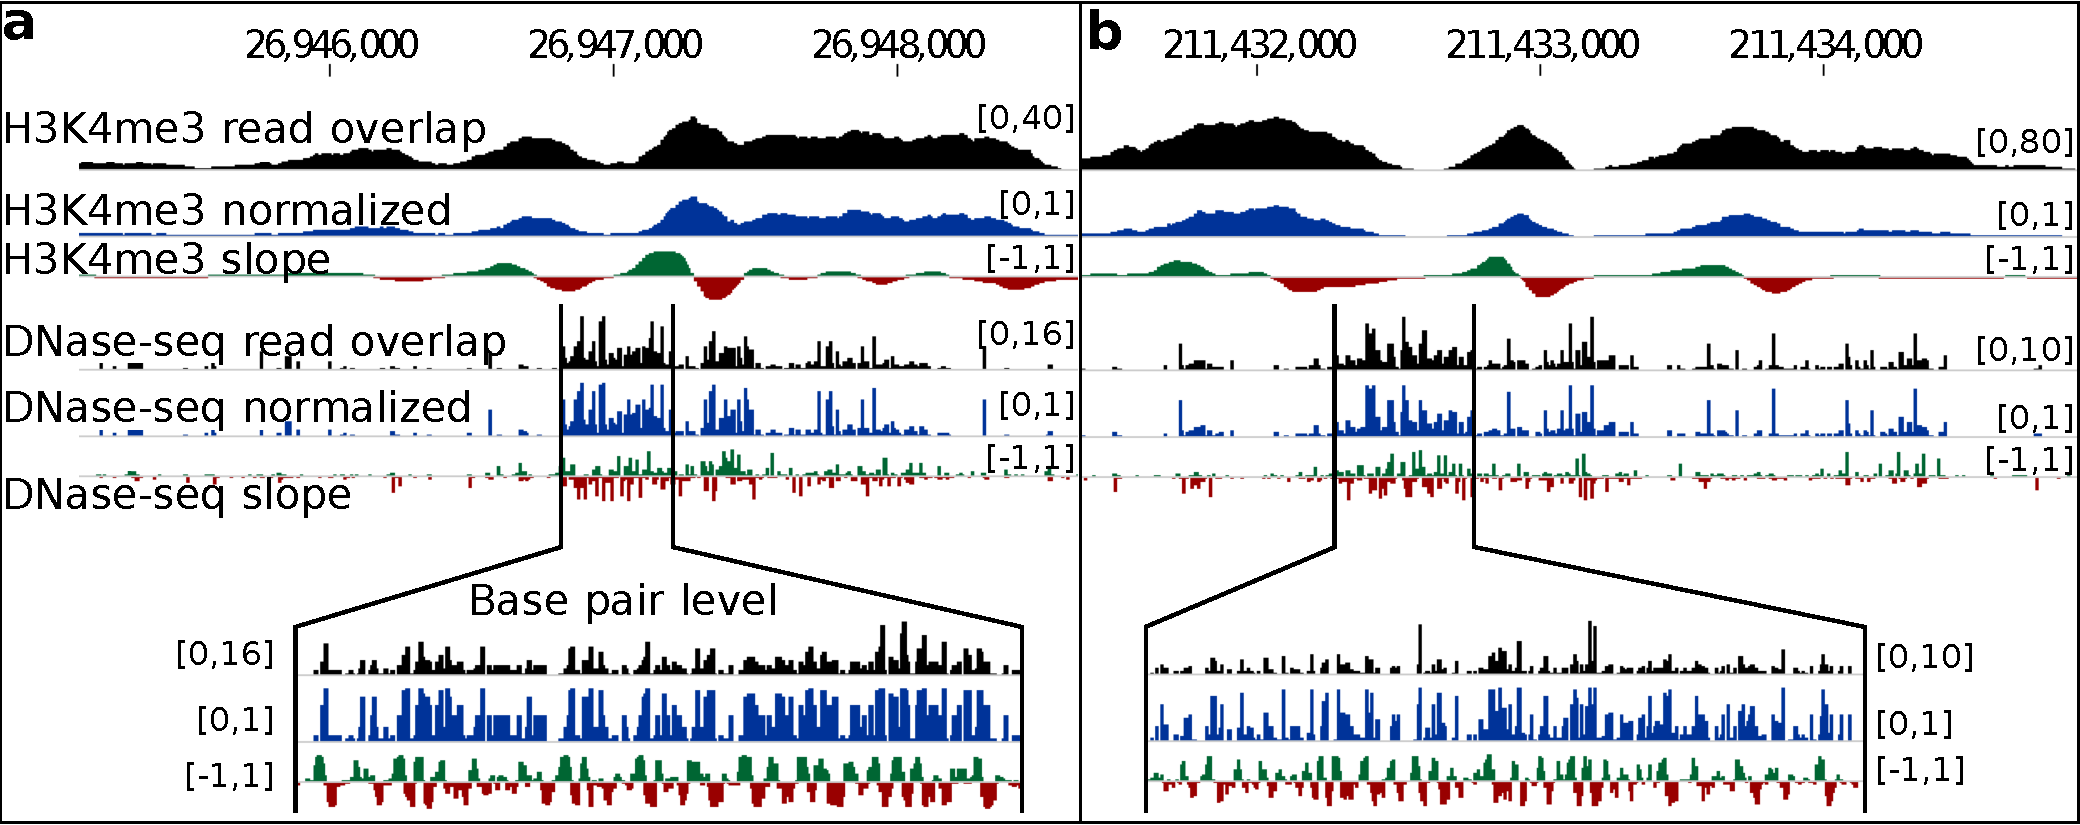
\includegraphics[width=0.99\textwidth]{gusmao_normslope}
\caption[Genomic signal treatment examples]{\textbf{Genomic signal treatment examples.} Examples of histone modification H3K4me3 ChIP-seq and DNase-seq signals before treatment (Counts), normalized (Normalized) and after Savitzky-Goaly smoothing and differentiation (Slope). In this figure we show examples for: (\textbf{a}) a promoter-proximal region and (\textbf{b}) a distal regulatory region. Both regions are from human chromosome~1.}
\label{fig:gusmao_normslope}
\end{figure}

%%%%%%%%%%%%%%%%%%%%%%%%%%%%%%%%%%%%%%%%%%%%%%%%%%%%%%%%%%%%%%%%%%%%%
% Section: Enriched Regions
%%%%%%%%%%%%%%%%%%%%%%%%%%%%%%%%%%%%%%%%%%%%%%%%%%%%%%%%%%%%%%%%%%%%%
\subsection{Enriched Regions}
\label{sec:enriched.regions}

% TODO



%%%%%%%%% DNASE

% DHS estimation using F-seq
DNase I hypersensitive sites (DHSs), i.e. regions enriched with DNase-seq cleavage activity, are estimated based on the DNase-seq raw signal $\mathbf{y}$. First, the F-seq software~\cite{boyle2008b} was used to create smoothed DNase-seq signals using Parzen density estimates. Then, the resulting smoothed signal $\mathbf{y^\text{fseq}}$ was fit to a gamma distribution,
\begin{equation}
  \label{eq:gamma}
  \mathbf{y^\text{fseq}} \sim \Gamma(\kappa,\theta),
\end{equation}
by evaluating $\kappa$ and $\theta$ based on mean and standard deviation estimates. Finally, the enriched regions (DHSs) were found by establishing a cutoff based on a $p$-value of $0.01$~\cite{boyle2008b,encode2012}.

We formally refer to DHSs as a set of genomic intervals
\begin{equation}
  \label{eq:dhs.set}
  H = \{{h}_{1}, ..., {h}_{L}\},
\end{equation}
where ${h}_{i} = [m,n]$ for $m<n \in \mathbb{N}$ and $L$ is the total number of DHSs. 

For simplicity of notation, we ignore the fact that intervals are defined on distinct chromosomes or contigs. In other words, we view the genome conceptually as a contiguous chain of genomic coordinates; despite the fact that it is actually divided into chromosomes.



%%%%%%%%%%%%%%%%%%%%%%%%%%%%%%%%%%%%%%%%%%%%%%%%%%%%%%%%%%%%%%%%%%%%%
% Section: Computational Footprinting with Hidden Markov Models
%%%%%%%%%%%%%%%%%%%%%%%%%%%%%%%%%%%%%%%%%%%%%%%%%%%%%%%%%%%%%%%%%%%%%
\section{Computational Footprinting with Hidden Markov Models}
\label{sec:computational.footprinting.hmm}

% Introductions
Hidden Markov model (HMMs) is a computational technique based on the Bayes probability theory and Markov stochastic processes. In this section we describe how we perform computational footprinting using HMMs. First, we formalize the HMM model and its parameters (Section~\ref{sec:multivariate.continuous.hmm}). Then, we describe how such model can be used to perform the computational footprinting using data from DNase-seq in combination with data from histone modification ChIP-seq signal (Section~\ref{sec:computational.footprinting.hmms}). Afterwards, we describe the processes used to train the HMM model (Section~\ref{sec:hmm.training}) and the algorithms used to perform the footprint predictions using the trained HMM model (Section~\ref{sec:hmm.decoding}). Finally, we discuss variations in our main model regarding the usage of only DNase-seq data or histone modification ChIP-seq data to perform the predictions (Section~\ref{sec:hmm.variations}). 

% Conclusion
The HMM theory and formalization presented here will be based on a number of publications~\cite{rabiner1989,durbin1998,mitchell1997,bishop2006,duda2000}. The discussion on how specific parameterizations were selected will take place in Section~\ref{sec:hmm.parameterization}. 

%%%%%%%%%%%%%%%%%%%%%%%%%%%%%%%%%%%%%%%%%%%%%%%%%%%%%%%%%%%%%%%%%%%%%
% Section: Multivariate Continuous HMM
%%%%%%%%%%%%%%%%%%%%%%%%%%%%%%%%%%%%%%%%%%%%%%%%%%%%%%%%%%%%%%%%%%%%%
\subsection{Multivariate Continuous HMM}
\label{sec:multivariate.continuous.hmm}

% Introduction
Markov chains are probabilistic models composed by a collection of states and transitions between these states, which correspond to the probability of changing between states. The hidden Markov models follow the same baseline idea, however they also contain within their model an unknown sequence of states associated to each input symbol. In this section we formalize the concept of hidden Markov models.

% Parameters
Let $\mathbf{X}^{D \times N}$ be a matrix of $D$ observed multivariate continuous genomic signals, each of which has length $N$, as described by equations~\ref{eq:multivar.matrix}--{eq:multivar.matrix.j}. For a given multivariate observation $\langle \mathbf{{x}_{\cdot 1}}, ..., \mathbf{{x}_{\cdot t}}, ..., \mathbf{{x}_{\cdot N}} \rangle$ from $\mathbf{X}$, we have a corresponding hidden sequence path $\mathbf{q} = \langle q_1, ..., q_t, ..., q_N \rangle$, where $ q_t \in \{1, ..., S\} $ represents the state emitting the vector $ \mathbf{{x}_{\cdot t}} $ at the $t^{\text{th}}$ genomic position. Then, we define a multivariate continuous HMM as the set of parameters
\begin{equation}
  \label{eq:hmm.theta}
  \Theta= \{\mathbf{A}, \mathbf{E}, \mathbf{s}\}.
\end{equation}

% Transitions
$\mathbf{A}$ represents the matrix which contains the mass probabilities of transitioning between the states of the HMM. We formalize this as
\begin{equation}
  \label{eq:hmm.a}
  \mathbf{A} = {\{a_{uv}\}}^{S \times S},
\end{equation}
where~$S$ is the number of states within the HMM topology and $a_{uv}$ represents the probability of transition from state $u$ to $v$, which is
\begin{equation}
  \label{eq:hmm.transition}
  a_{uv} = P(q_t = v | q_{t-1} = u).
\end{equation}

% Emission
$\mathbf{E}$ represents the set of emission probabilities. We define $\mathbf{E}$ as a vector of probability density functions
\begin{equation}
  \label{eq:hmm.e}
  \mathbf{E} = \langle e_1(\mathbf{b}), ..., e_S(\mathbf{b}) \rangle,
\end{equation}
where each state $u$ has a probability $e_u(\mathbf{b})$ of emitting the vector symbol $ \mathbf{b} $. Such probability density function is represented by
\begin{equation}
  \label{eq:hmm.emission}
  e_u(\mathbf{x}) = p(\mathbf{{x}_{\cdot t}} = \mathbf{b} | q_t = u).
\end{equation}
The probability density function used for the emission probabilities correspond to a multivariate normal density function with full covariance matrix. This is described as
\begin{equation}
  \label{eq:hmm.emission.gaussian}
  \begin{array}{lcl}
    p(\mathbf{{x}_{\cdot t}} = \mathbf{b} | q_t = u) & = & 
    p(\mathbf{x_{\cdot t}}|{{\boldsymbol\mu}^{\mathbf{u}}},{{\boldsymbol\Sigma}^{\mathbf{u}}})\\[0.4em] & = &
    \frac{1}{ \sqrt{(2\pi)^{D} {| {{\boldsymbol\Sigma}^{\mathbf{u}}} |}}}
    e^{-\frac{1}{2} (\mathbf{x_{\cdot t}}-{{\boldsymbol\mu}^{\mathbf{u}}})^T ({{\boldsymbol\Sigma}^{\mathbf{u}}})^{-1} (\mathbf{x_{\cdot t}}-{{\boldsymbol\mu}^{\mathbf{u}}})}, \\
  \end{array}
\end{equation}
where ${{\boldsymbol\mu}^{\mathbf{u}}}$ and ${{\boldsymbol\Sigma}^{\mathbf{u}}}$ are, respectively, the $D$-dimensional mean vector and full covariance matrix of the emission probability density function at state $u$.

% Initial state probabilities
$\mathbf{s}$ represents the initial set of transition probabilities. Such parameter is required to ``start'' the model at a given set of states. The initial state transition probabilities are represented as a vector of mass probabilities
\begin{equation}
  \label{eq:hmm.initial}
  \mathbf{s} = \langle s_{1}, ..., s_{S} \rangle.
\end{equation}

% Independence assumptions
There are two independence assumptions which need to be made in order to be able to work with the aforementioned proposed HMM. The first assumption is that the probability to reach state $t$ depends only on the previous state $t-1$
\begin{equation}
  \label{eq:hmm.indep.1}
  p(q_t | q_1, ..., q_{t-1}) = p(q_t | q_{t-1}),
\end{equation}
and the second assumption dictates that the density function of emitting an input vector $\mathbf{{x}_{\cdot t}}$ observed at state $t$, depends only at this current state
\begin{equation}
  \label{eq:hmm.indep.2}
  p(\mathbf{{x}_{\cdot t}} | q_1, ..., q_t) = p(\mathbf{{x}_{\cdot t}} | q_t).
\end{equation}

% HMM problems - intuition 1
Given the formalism previously defined, there are three general problems on which we can address directly through computationally efficient implementations of HMMs:

\begin{center}
  \begin{tabular}{lp{.8\linewidth}}
    {\bf Problem 1} & Estimate the HMM parameters $ \Theta $ in order to maximize $p(\mathbf{X} | \Theta)$. \\[0.2cm]
    {\bf Problem 2} & Given an observed multivariate input $ \mathbf{X} $ and an HMM model represented by the parameters $ \Theta $, find the sequence of hidden states $ \mathbf{q} $ which best explains the input given the HMM model, i.e. that maximizes $ p\left( \mathbf{X}, \mathbf{q} | \Theta \right) $ . \\[0.2cm]
    {\bf Problem 3} & Given an observed multivariate input $ \mathbf{X} $ and an HMM model represented by the parameters $ \Theta $, compute the probability of the input sequence given the HMM model $p(\mathbf{X} | \Theta)$. \\[0.2cm]
  \end{tabular}
\end{center}

% HMM problems - intuition 2
The first problem regards the HMM parameter estimation, i.e. model training. This problem will be addressed in Section~\ref{sec:hmm.training}. The second and third problems represent our genomic segmentation methodology using the HMM states in order to predict active binding sites. These problems will be explored in Section~\ref{sec:hmm.decoding}.

%%%%%%%%%%%%%%%%%%%%%%%%%%%%%%%%%%%%%%%%%%%%%%%%%%%%%%%%%%%%%%%%%%%%%
% Section: Computational Footprinting with HMMs
%%%%%%%%%%%%%%%%%%%%%%%%%%%%%%%%%%%%%%%%%%%%%%%%%%%%%%%%%%%%%%%%%%%%%
\subsection{Computational Footprinting with HMMs}
\label{sec:computational.footprinting.hmms}

% Signal input
The HMM structure (topology of states) was designed to recognize the epigenetic grammar described in Section~\ref{sec:grammar.tfbs}. This segmentation task is performed based on four input signals: the normalized and slope versions of both DNase-seq and a histone modification ChIP-seq. In formal terms, our input matrix $\mathbf{X}$ can be represented as
\begin{equation}
  \label{eq:signal.matrix}
  \mathbf{X} = 
  \begin{pmatrix}
    x^{\text{norm}}_{\text{dnase},1} & x^{\text{norm}}_{\text{dnase},2} & \dots & x^{\text{norm}}_{\text{dnase},N} \\[1em]
    x^{\text{slope}}_{\text{dnase},1} & x^{\text{slope}}_{\text{dnase},2} & \dots & x^{\text{slope}}_{\text{dnase},N} \\[1em]
    x^{\text{norm}}_{\text{histone},1} & x^{\text{norm}}_{\text{histone},2} & \dots & x^{\text{norm}}_{\text{histone},N} \\[1em]
    x^{\text{slope}}_{\text{histone},1} & x^{\text{slope}}_{\text{histone},2} & \dots & x^{\text{slope}}_{\text{histone},N} \\
  \end{pmatrix}.
\end{equation}

% Segmentation goal
An example of the signal defined in Equation~\ref{eq:signal.matrix} can be seen in Figure~\ref{fig:gusmao_hmm_footprinting}a. The goal of our HMM model is to segment this region with regard to the level of both DNase-seq and histone modification ChIP-seq. For that, we devised the HMM topology graphically depicted in Figure~\ref{fig:gusmao_hmm_footprinting}b, which can be interpreted as follows.

% HMM topology
The first state ({\tt BACK}) corresponds to the ``background'' regions with low concentration of DNase-seq and histone modification ChIP-seq signals. The histone level states represent a peak in the histone modification ChIP-seq signal, recognizing an increase in the histone modification ChIP-seq signal based on high positive $x^{\text{slope}}_{\text{histone},\cdot}$ values ({\tt UP}), summit regions with $x^{\text{slope}}_{\text{histone},\cdot}$ values close to zero with high $x^{\text{norm}}_{\text{histone},\cdot}$ values ({\tt TOP}) and a decrease based on negative values of the $x^{\text{slope}}_{\text{histone},\cdot}$ signal ({\tt DOWN}). From the histone level {\tt DOWN} state, the model can either return to {\tt BACK} (isolated histone modification peaks without further DHSs) or continue to the DNase level {\tt UP} state. The DNase level states are equivalent to the histone level states, with the exception that the $x^{\text{norm}}_{\text{dnase},\cdot}$ and $x^{\text{slope}}_{\text{dnase},\cdot}$ signals are being recognized instead. From the DNase level {\tt DOWN} state, the model decides between returning to a region of higher histone modification ChIP-seq signals (histone level {\tt UP} state) and visiting the {\tt FOOTPRINT} state, which represents the dip between two peaks of intense DNase I cleavage. The regions of the genome where the HMM has recognized as {\tt FOOTPRINT} are the ones reported by our method as likely TFBSs.

% Different histone modifications
It is clear now that our computational footprinting HMM requires one DNase-seq signal and one histone modification ChIP-seq signal in order to form our input matrix. In this work, we tested different histone modifications which indicate active regulatory regions. The histone modifications H3K4me3, H3K9ac, H3K27ac and H2A.Z usually happen in proximal regulatory regions. Furthermore, we also used the histone modification H3K4me1, which usually demarks distal regulatory regions.

% Alternative topologies
We will explore alternative topologies regarding the usage of a different input signal matrix $\mathbf{X}$ in Section~\ref{sec:hmm.variations}. Also, we will explore alternative topologies with regard to simplified HMM models in Section~\ref{sec:alternative.topologies}.

% Figure - Computational footprinting with HMMs
\begin{figure}[h!]
\centering
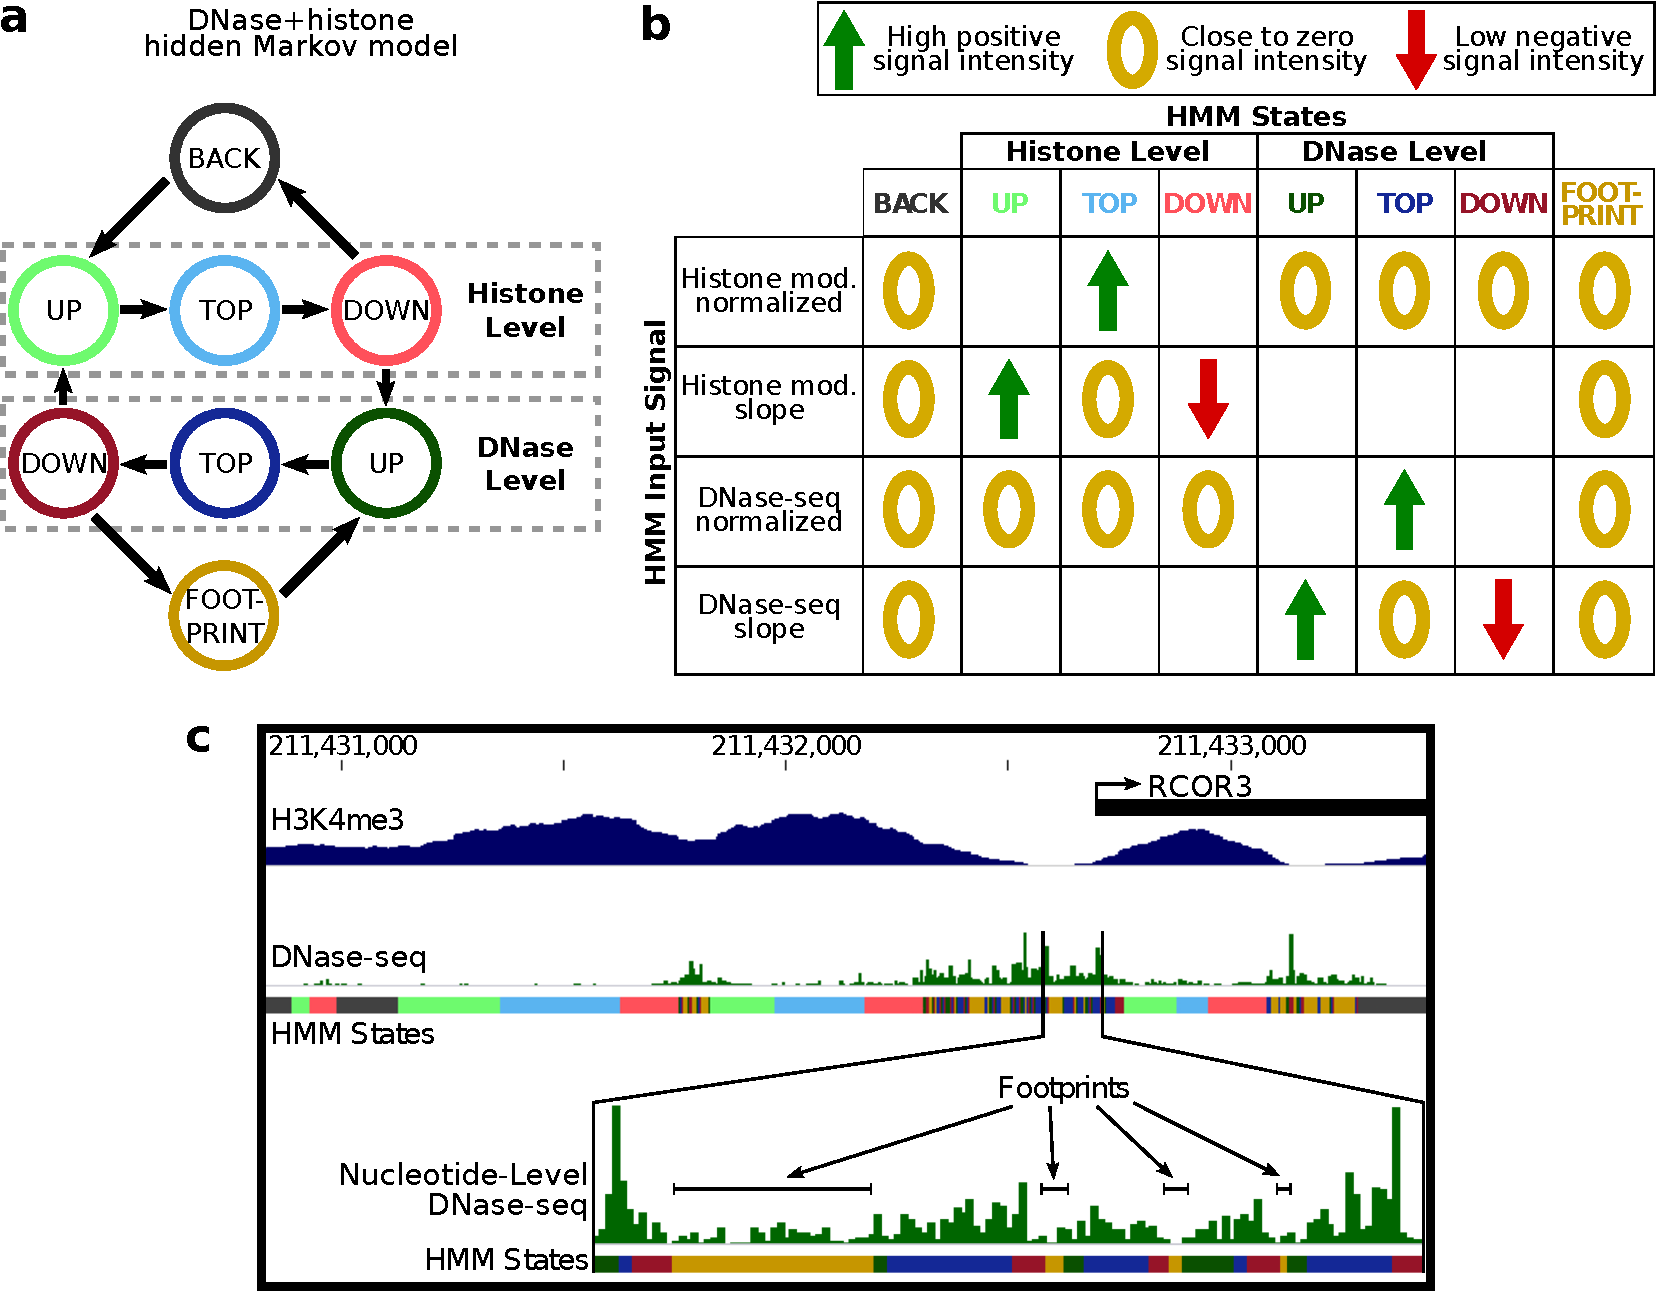
\includegraphics[width=0.99\textwidth]{gusmao_hmm_footprinting}
\caption[Computational footprinting with HMMs]{\textbf{Computational footprinting with HMMs.} (\textbf{a}) DNase-seq and H3K4me3 (ChIP-seq) profiles around the promoter region of RCOR3 -- REST corepressor 3 on K562 cell type. The DNase-seq signal indicates three clear DHSs (HS1, HS2 and HS3), each of which fits dip regions within the H3K4me3 signal. Moreover, these regions consist of several putative footprints of varied sizes. (\textbf{b}) Eight state HMM proposed. The first state models background signal ({\tt BACK}). From the background state, the only possible transition is to the histone level states, which will model the increase ({\tt UP}), high levels ({\tt TOP}) and decrease ({\tt DOWN}) of histone modifications. After visiting histone level states, the HMM allows transitions to the DNase level states, which again model the increase, high levels and decrease in the DHS signal. Only then, the {\tt FOOTPRINT} state can be visited. After a footprint visit, the HMM has to go again to the DNase and histone level states, emphasizing the peak-dip-peak pattern. We omit the self-transitions, which are present in all states, for simplicity.}
\label{fig:gusmao_hmm_footprinting}
\end{figure}

%%%%%%%%%%%%%%%%%%%%%%%%%%%%%%%%%%%%%%%%%%%%%%%%%%%%%%%%%%%%%%%%%%%%%
% Section: HMM Training
%%%%%%%%%%%%%%%%%%%%%%%%%%%%%%%%%%%%%%%%%%%%%%%%%%%%%%%%%%%%%%%%%%%%%
\subsection{HMM Training}
\label{sec:hmm.training}

% Introduction
In this work, we estimated the HMM parameters in a supervised manner, using the maximum likelihood method. Alternatively, HMM parameters can be estimated in an unsupervised approach using the Baum-Welch algorithm. Preliminary tests on using the Baum-Welch algorithm did not provide consistent results~\cite{gusmao2012}. Therefore, in this work, we will focus only on the suppervised approach for simplicity.

% Manual annotation - region selection
We selected a $10,000$ bp region (with genomic coordinates $211,428,000--211,438,000$ in human chromosome~1) around the promoter of the gene RCOR3 and performed a cell-specific manual annotation, in which each genomic position is assigned with a state from our $8$-state HMM topology, following the epigenetic grammar described in Figure~\ref{fig:gusmao_grammar_tfbs}. This promoter-proximal regulatory region annotated with HMM states was used to train the models which use histone modifications H3K4me3, H3K9ac, H3K27ac and H2A.Z. As the histone modification H3K4me1 is known to be associated to distal regulatory regions, we have additionally annotated an enhancer region (with genomic coordinates $26,942,000--26,952,000$ in human chromosome~1). The selection of these regions was made randomly, but we checked ENCODE~\cite{encode2012} tracks for evidence that the gene RCOR3 was expressed in all cell types analyzed and that the enhancer region was far ($>100$ kb) from known genes and expressed regions but associated with the expression of the closest gene's transcription start site.

% Manual annotation - process
In order to help the annotation of the footprints, MPBSs obtained by applying motif matching with all PFMs from Jaspar~\cite{mathelier2014}, Uniprobe~\cite{robasky2011} and Transfac~\cite{matys2006} PFM repositories were detected inside the training regions. We consider ``real'' footprints all the DNase-seq signal depleted regions between two DNase-seq peaks that overlap a MPBS. We trained five HMMs per cell type, one for each histone modification (H3K4me3, H3K9ac, H3K29ac and H2A.Z with the promoter-proximal regulatory region and H3K4me1 with the distal regulatory region). The regions used for training were excluded from all further predictions.

% Training A
For a given annotation sequence of the HMM states $\mathbf{q}$ and sample data $\mathbf{X}$, the transition mass probabilities can be estimated as
\begin{equation}
  \label{eq:hmm.train.a.1}
  a_{uv} = \frac{ \alpha^{\prime}_{uv}}{ \sum_{w=1}^{S} \alpha^{\prime}_{uw}},
\end{equation}
where $ \alpha^{\prime}_{uv} $ represents the number of transitions from state~$u$ to state~$v$ observed in the annotated training data, formally defined as
\begin{equation}
  \label{eq:hmm.train.a.2}
  \alpha^{\prime}_{uv} = \sum_i^{N-1} \mathbf{1} (q_i=u,q_{i+1}=v),
\end{equation}
where $ {\mathbf{1}}(\cdot) $ denotes the indicator function.

% Training E
The emission probability density functions (gaussians) are estimated as
\begin{equation}
  \label{eq:hmm.train.e.1}
  \mu^{u}_{i} = \frac{ \sum_{j=1}^{N} {x}_{ij} {\mathbf{1}}(q_j=u) }{ \sum_{j=1}^{N} {\mathbf{1}} (q_j=u) },
\end{equation}
where $ \mu^{u}_{i} $ is the gaussian's mean at state $u$ for the signal $i$ and
\begin{equation}
  \label{eq:hmm.train.e.2}
  {\sigma}^{u}_{ik} = \frac{\sum_{j=1}^{N} ({x}_{ij} - \mu^{u}_{i})^T({x}_{kj} - \mu^{u}_{k}) {\mathbf{1}} (q_j=u)}
  {\sum_{j=1}^{N} {\mathbf{1}} (q_j=u) - 1}.
\end{equation}
where $ \sigma^{u}_{ik} $ is the gaussian's variance at state $u$ between signals $i$ and $k$.

% Training s
As we expect the HMM to always start at the {\tt BACK} state (the first HMM state), the initial transition vector $\mathbf{s}$ was manually set with the following probabilities
\begin{equation}
  \label{eq:hmm.train.s}
  \begin{array}{lcl}
    s_1 = 1 \\
    s_t = 0 \quad \forall \quad t \neq 1 \\
  \end{array}.
\end{equation}

% Example of HMM parameters
Here we show an example of a complete set of HMM parameters, regarding the model trained with DNase-seq $+$ H3K4me3 using data from the H1-hESC cell. The Table~\ref{tab:hmmtrans} represents the transition matrix. Each number represents the probability of performing a transition from the HMM state in the first column of the entry's row to the HMM state in the first row of the entry's column. The Table~\ref{tab:hmmmean} exhibits the emission distribution mean values. It contains the mean in which each signal type (represented in the columns) assumes at each state (represented in the rows). Finally, the Table~\ref{tab:hmmcov} shows all covariance matrices from the emission distributions. The full covariance matrix is depicted for each state, in which rows and columns are sorted by the input signals: DNase normalized, DNase slope, H3K4me3 normalized and H3K4me3 slope.

\begin{table}[t]
\footnotesize
\begin{center}
\caption{Transition probabilities of the HMM trained with H3K4me3 using H1-hESC data. Transitions are specified from the states in the rows to the states in the columns. Histone level states are denoted with `(H)' and DNase level states with `(D)'. The {\tt FOOTPRINT} state is abreviated as `FP'.}
\label{tab:hmmtrans}
    \renewcommand{\arraystretch}{1.2}
    \begin{tabular}{ lllllllll }
        \hline
        & \textbf{BACK} & \textbf{UP (H)} & \textbf{TOP (H)} & \textbf{DOWN (H)} & \textbf{UP (D)}
        & \textbf{TOP (D)} & \textbf{DOWN (D)} & \textbf{FP} \\
        \textbf{BACK}     & 0.9997 & 0.0003 & 0.0    & 0.0    & 0.0    & 0.0    & 0.0   & 0.0    \\
        \textbf{UP (H)}   & 0.0    & 0.9915 & 0.0085 & 0.0    & 0.0    & 0.0    & 0.0   & 0.0    \\
        \textbf{TOP (H)}  & 0.0    & 0.0    & 0.9901 & 0.0099 & 0.0    & 0.0    & 0.0   & 0.0    \\
        \textbf{DOWN (H)} & 0.0057 & 0.0    & 0.0    & 0.9861 & 0.0082 & 0.0    & 0.0   & 0.0    \\
        \textbf{UP (D)}   & 0.0    & 0.0    & 0.0    & 0.0    & 0.6515 & 0.3485 & 0.0   & 0.0    \\
        \textbf{TOP (D)}  & 0.0    & 0.0    & 0.0    & 0.0    & 0.0    & 0.783  & 0.217 & 0.0    \\
        \textbf{DOWN (D)} & 0.0    & 0.0339 & 0.0    & 0.0    & 0.0    & 0.0    & 0.577 & 0.3891 \\
        \textbf{FP}       & 0.0    & 0.0    & 0.0    & 0.0    & 0.0564 & 0.0    & 0.0   & 0.9436 \\
        \hline
    \end{tabular}
\end{center}
\end{table}

\begin{table}[t]
\footnotesize
\begin{center}
\caption{Signals' mean values for each state of the HMM trained with H3K4me3 using H1-hESC data. Histone level states are denoted with `(H)' and DNase level states with `(D)'. The {\tt FOOTPRINT} state is abreviated as `FP'.}
\label{tab:hmmmean}
    \renewcommand{\arraystretch}{1.2}
    \begin{tabular}{ lllll }
        \hline
        & \textbf{DNase norm.} & \textbf{DNase slope} & \textbf{Histone norm.} & \textbf{Histone slope} \\
        \textbf{BACK}     & 0.0045 & -0.0002 & 0.0441 & 0.0007  \\
        \textbf{UP (H)}   & 0.0501 & 0.0043  & 0.1983 & 0.2995  \\
        \textbf{TOP (H)}  & 0.0445 & -0.0075 & 0.4693 & 0.0158  \\
        \textbf{DOWN (H)} & 0.0636 & 0.0003  & 0.2309 & -0.4237 \\
        \textbf{UP (D)}   & 0.1537 & 0.6343  & 0.0894 & -0.0647 \\
        \textbf{TOP (D)}  & 0.4244 & 0.0059  & 0.1091 & -0.0735 \\
        \textbf{DOWN (D)} & 0.1578 & -0.6562 & 0.0816 & -0.0434 \\
        \textbf{FP}       & 0.0902 & -0.0162 & 0.1009 & -0.0436 \\
        \hline
    \end{tabular}
\end{center}
\end{table}

\begin{table}[t]
\footnotesize
\begin{center}
\caption{Covariance matrices for each state of the HMM trained with H3K4me3 using H1-hESC data. Within each state's matrix, lines and rows are sorted by signal type as DNase normalized, DNase slope, H3K4me3 normalized and H3K4me3 slope. Histone level states are denoted with `(H)' and DNase level states with `(D)'. The {\tt FOOTPRINT} state is abreviated as `FP'.}
\label{tab:hmmcov}
    \renewcommand{\arraystretch}{1.2}
    \begin{tabular}{>{\centering\arraybackslash} m{0.2cm}
                    >{\centering\arraybackslash} m{1.2cm}
                    >{\centering\arraybackslash} m{1.2cm}
                    >{\centering\arraybackslash} m{1.2cm}
                    >{\centering\arraybackslash} m{1.2cm}|
                    >{\centering\arraybackslash} m{0.2cm}
                    >{\centering\arraybackslash} m{1.2cm}
                    >{\centering\arraybackslash} m{1.2cm}
                    >{\centering\arraybackslash} m{1.2cm}
                    >{\centering\arraybackslash} m{1.2cm} }
        \hline
        \multirow{4}{*}{\rotatebox[origin=c]{90}{\textbf{BACK}}}
        & 0.0025  & -0.0001 & 0.0001 & 0.0    &
        \multirow{4}{*}{\rotatebox[origin=c]{90}{\textbf{UP (H)}}}
        & 0.0222  & 0.0001  & 0.003  & 0.0057 \\
        & -0.0001 & 0.0025  & 0.0    & 0.0    &
        & 0.0001  & 0.0155  & 0.0006 & 0.0005 \\
        & 0.0001  & 0.0     & 0.0047 & 0.0    &
        & 0.003   & 0.0006  & 0.0101 & 0.0105 \\
        & 0.0     & 0.0     & 0.0    & 0.0019 &
        & 0.0057  & 0.0005  & 0.0105 & 0.0341 \\
        \hline
        \multirow{4}{*}{\rotatebox[origin=c]{90}{\textbf{TOP (H)}}}
        & 0.0216  & 0.0003  & -0.0009 & 0.0014  &
        \multirow{4}{*}{\rotatebox[origin=c]{90}{\textbf{DOWN (H)}}}
        & 0.0239  & 0.0001  & -0.0033 & -0.0002 \\
        & 0.0003  & 0.0196  & 0.0005  & 0.0003  &
        & 0.0001  & 0.009   & 0.0002  & -0.0006 \\
        & -0.0009 & 0.0005  & 0.0047  & -0.001  &
        & -0.0033 & 0.0002  & 0.0156  & -0.0095 \\
        & 0.0014  & 0.0003  & -0.001  & 0.0193  &
        & -0.0002 & -0.0006 & -0.0095 & 0.0313  \\
        \hline
        \multirow{4}{*}{\rotatebox[origin=c]{90}{\textbf{UP (D)}}}
        & 0.0705  & 0.0246  & -0.0053 & 0.0025  &
        \multirow{4}{*}{\rotatebox[origin=c]{90}{\textbf{TOP (D)}}}
        & 0.1559  & -0.002  & -0.0079 & 0.0052  \\
        & 0.0246  & 0.0714  & -0.0038 & -0.0015 &
        & -0.002  & 0.0384  & -0.0008 & 0.0021  \\
        & -0.0053 & -0.0038 & 0.0045  & -0.0056 &
        & -0.0079 & -0.0008 & 0.007   & -0.0096 \\
        & 0.0025  & -0.0015 & -0.0056 & 0.0125  &
        & 0.0052  & 0.0021  & -0.0096 & 0.0184  \\
        \hline
        \multirow{4}{*}{\rotatebox[origin=c]{90}{\textbf{DOWN (D)}}}
        & 0.0687  & -0.011  & -0.0048 & 0.004   &
        \multirow{4}{*}{\rotatebox[origin=c]{90}{\textbf{FP}}}
        & 0.0358  & -0.0019 & -0.0025 & 0.0007  \\
        & -0.011  & 0.055   & 0.0039  & -0.0    &
        & -0.0019 & 0.0225  & 0.0001  & 0.0002  \\
        & -0.0048 & 0.0039  & 0.0039  & -0.0044 &
        & -0.0025 & 0.0001  & 0.0068  & -0.0069 \\
        & 0.004   & -0.0    & -0.0044 & 0.0109  &
        & 0.0007  & 0.0002  & -0.0069 & 0.0121  \\
        \hline
    \end{tabular}
\end{center}
\end{table}

%%%%%%%%%%%%%%%%%%%%%%%%%%%%%%%%%%%%%%%%%%%%%%%%%%%%%%%%%%%%%%%%%%%%%
% Section: HMM Decoding
%%%%%%%%%%%%%%%%%%%%%%%%%%%%%%%%%%%%%%%%%%%%%%%%%%%%%%%%%%%%%%%%%%%%%
\subsection{HMM Decoding}
\label{sec:hmm.decoding}

% Introduction
Given an HMM with parameters estimated as described in Section~\ref{sec:hmm.training} we are able to perform the prediction of active transcription factor binding sites. First, we reduce the number of genomic regions in which we apply the HMM decoding algorithms by selecting only the regions enriched for the particular signals being analyzed (Section~\ref{sec:selection.genomic.regions}). Then, we can predict active TFBSs using two approaches which are computationally feasible. The first -- termed Viterbi algorithm -- address the {\bf Problem 2} defined in Section~\ref{sec:multivariate.continuous.hmm}. Briefly, it computes the sequence of hidden states $ \mathbf{q} $ that maximizes $ p\left( \mathbf{X}, \mathbf{q} | \Theta \right) $. Then, given the computated sequence of hidden states we are able to identify the ones which corresponds to the {\tt FOOTPRINT} state and regard these regions as the active transcription factor binding sites. This algorithm will be described in Section~\ref{sec:viterbi.algorithm}. Furthermore, we can address the {\bf Problem 3} defined in Section~\ref{sec:multivariate.continuous.hmm} and compute the posterior probability $ p(q_i = u | \mathbf{X}, \Theta) $ of being in a certain state $u$ (in this case, we are interested in the {\tt FOOTPRINT} state) at a certain time $t$ given the input signal $\mathbf{X}$ and the HMM parameters $\Theta$. This approach will be described in Section~\ref{sec:posterior.probability}.

%%%%%%%%%%%%%%%%%%%%%%%%%%%%%%%%%%%%%%%%%%%%%%%%%%%%%%%%%%%%%%%%%%%%%
% Section: Selection of Genomic Regions
%%%%%%%%%%%%%%%%%%%%%%%%%%%%%%%%%%%%%%%%%%%%%%%%%%%%%%%%%%%%%%%%%%%%%
\subsubsection{Selection of Genomic Regions}
\label{sec:selection.genomic.regions}

% Selection of genomic regions
To reduce the dimensionality of the data, we first applied a peak calling tool to find regions enriched with either DNase-seq and histone modification ChIP-seq signals. The enriched regions of histone modifications ChIP-seq data were defined using the peak-calling tool MACS~\cite{zhang2008}. We used a lenient $p$-value of $ 10^{-5} $ and all default parameters from MACS version $1.4$. No further filtering was performed on the resulting histone modification peaks, as we wanted a lenient selection of candidate regions. The enriched regions of the DNase-seq data were defined as in~\cite{boyle2011}. Briefly, a signal corresponding to the estimated density of the DHS is generated by applying F-seq software~\cite{boyle2008b} to the DNase-seq mapped reads and background information based on alignability, copy number and karyotype correction. A threshold is then calculated by fitting the signal to a gamma distribution and considering the value that corresponds to a loose $p$-value of $ 0.01 $ (same procedure as described in Section~\ref{sec:dnase.hypersensitive.sites}). We merge all enriched regions for a given cell type and extend them by $5,000$ bp in each direction. This step keeps only $3-6\%$ of the genome with DNase-seq or histone modification ChIP-seq evidence for a given cell type.

% Mathematical definition of input
In the following subsections we will describe the computational footprinting using the Viterbi algorithm and the posterior probability decoding. In these cases, for simplicity, we will define the input matrix as $ \mathbf{X} $. Such matrix of length $ N $ correspond to a single region obtained with the aforementioned procedure of selecting enriched genomic regions. The complete footprinting process consists on applying the algorithms that will be described in the following subsections in all the enriched genomic regions, one at a time. Such procedure was optimized by using the computational parallelization approach described in the Python package \emph{multiprocessing}.

%%%%%%%%%%%%%%%%%%%%%%%%%%%%%%%%%%%%%%%%%%%%%%%%%%%%%%%%%%%%%%%%%%%%%
% Section: Viterbi Algorithm
%%%%%%%%%%%%%%%%%%%%%%%%%%%%%%%%%%%%%%%%%%%%%%%%%%%%%%%%%%%%%%%%%%%%%
\subsubsection{Viterbi Algorithm}
\label{sec:viterbi.algorithm}

% Introduction
As previously mentioned, we are interested on identifying the most probable path $ \mathbf{q^*} $ given the input $ \mathbf{X} $ on an HMM $ \Theta $. In formal terms, we are interested in evaluating the follwing equation
\begin{equation}
  \label{eq:viterbi1}
  \mathbf{q^*} = \argmax{\mathbf{q}} p\left(\mathbf{X}, \mathbf{q} | \Theta \right).
\end{equation}

% Exponential problem - viterbi solution
The solution to the equation~\ref{eq:viterbi1} can be found in an exaustive way by evaluating $ p\left(\mathbf{X}, \mathbf{q} | \Theta \right) $ for all $ S^N $ possible instances of the $N$-length vector $ \mathbf{q} $, in which each element assumes one of the $S$ HMM states. It is clear, however, that the complexity of such approach, in terms of the big-$\mathcal{O}$ notation is $ \mathcal{O}(S^N) $, i.e. it grows exponentially given the input vector with length $N$. Fortunately, it is possible to solve the equation~\ref{eq:viterbi1} using a dynamic programming algorithm which relies on the HMM independence claims described by equations~\ref{eq:hmm.indep.1} and~\ref{eq:hmm.indep.2} with a polynomial complexity $ \mathcal{O}(N \times S^2) $ using the Viterbi algorithm.

% Introdução - viterbi
The Viterbi algorithm was proposed by Andrew Viterbi in 1976 as a decoding algorithm for convolutional codes over digital telecommunication connections that contained a high level of noise. After its proposition, such algorithm was aplied in various areas such as digital mobile phone signal processing, dial-up modems, satelites, wireless networks and currently is heavily explored by machine learning areas such as pattern recognition, computational linguistics and bioinformatics~\cite{rabiner1989}. In the following we will describe the Viterbi algorithm.

% Viterbi variable
Let $ \nu_u(t) $ be a Viterbi variable, which corresponds to the probability of the most probable path of the input subset $ \langle \mathbf{{x}_{\cdot 1}}, ..., \mathbf{{x}_{\cdot t}} \rangle $ ending at state $ u $. Assuming knowledge of $ \nu_u(t) $, we are able to evaluate the probability for the path subset $ \langle \mathbf{{x}_{\cdot 1}}, ..., \mathbf{{x}_{\cdot t+1}} \rangle $ using the HMM independence claims as
\begin{equation}
  \label{eq:viterbi2}
  \nu_v(t+1) = e_v(\mathbf{{x}_{\cdot t+1}}) {max}_u(\nu_u(t) a_{uv})
\end{equation}

% Viterbi algorithm - description
Given that we start our HMM decoding at a figurative initial time $ 0 $, we can define the initial Viterbi variables for all HMM states as our initial HMM probabilities (equation~\ref{eq:hmm.initial}) as
\begin{equation}
  \label{eq:viterbi3}
  \nu_u(0) = s_u.
\end{equation}
From this initial time we are able to calculate the viterbi variables for all the following input time points using equation~\ref{eq:viterbi2}. Furthermore, we can dinamically construct a ``pointer'' vector $\boldsymbol\phi$ in which we add the most probable states in each iteration of viterbi variable calculations for the following input time points. The algorithm is fully described as follows. In the following algorithm we denote as $ \varepsilon $ an additional figurative last state of our path $ \mathbf{q} $ in order to formally describe the algorithm termination.

% Viterbi algorithm
\begin{center}
  \begin{spacing}{1.0}
    \begin{tabular}{l}
      \hline \\[-0.25cm]
      \hspace{1.2cm} {\large {\bf \emph{ Viterbi Algorithm } } } \hspace{1.2cm} \\[0.1cm]
      \hline \\[-0.25cm]
      \hspace{0.2cm} {\bf 1. Initialization:} \\
      \hspace{0.9cm} 1.1. $ \nu_u(0) = s_u $ \\
      \hspace{0.2cm} {\bf 2. Iteration $ (t = 1, ..., N) $:} \\
      \hspace{0.9cm} 2.1. $ \nu_v(t) = e_v(\mathbf{{x}_{\cdot t}}) {max}_u(\nu_u(t-1)a_{uv}) $ \\
      \hspace{0.9cm} 2.2. $ {\phi}_{v}(t) = {argmax}_u(\nu_u(t-1)a_{uv}) $ \\
      \hspace{0.2cm} {\bf 3. Termination:} \\
      \hspace{0.9cm} 3.1. $ p(\mathbf{X},\mathbf{q^*}) = {max}_u(\nu_u(N)a_{u\varepsilon}) $ \\
      \hspace{0.9cm} 3.2. $ q_{N}^{\ast} = {argmax}_u(\nu_u(N)a_{u\varepsilon}) $ \\
      \hspace{0.2cm} {\bf 4. Reassembly $ (t = N, ..., 1) $:} \\
      \hspace{0.9cm} 4.1. $ q_{t-1}^{\ast} = {\phi}_{q_{t}^{\ast}}(t) $ \\[0.1cm]
      \hline
    \end{tabular}
  \end{spacing}
\end{center}

% Practical terms
The identification of active transcription factor binding sites (footprints) can be performed evaluating all genomic positions $t$ in which the predicted hidden state $ q_t = \text{{\tt FOOTPRINT}} $. The contiguous genomic regions are merged and extended by $3$ bps for each side. Such extension is necessary in order to correct for the discrepancy between the short footprint sizes in relation to the TF affinity sequences~\cite{boyle2011,gusmao2014}.

%%%%%%%%%%%%%%%%%%%%%%%%%%%%%%%%%%%%%%%%%%%%%%%%%%%%%%%%%%%%%%%%%%%%%
% Section: Posterior Probability
%%%%%%%%%%%%%%%%%%%%%%%%%%%%%%%%%%%%%%%%%%%%%%%%%%%%%%%%%%%%%%%%%%%%%
\subsubsection{Posterior Probability}
\label{sec:posterior.probability}

% Bayes posterior probability
The posterior probability can be defined as the probability of observing the hidden state $ u $ at a certain input time. It can be formally defined using Bayes theorem as
\begin{equation}
  \label{eq:posterior1}
  p(q_t = u | \mathbf{X}) = \frac{p(\mathbf{X}, q_t = u)}{p(\mathbf{X})}.
\end{equation}

% Evidence probability
First, we focus on the evaluation of the clause $ p(\mathbf{X}) $ from equation~\ref{eq:posterior1}, which is the probability of a certain input matrix $ \mathbf{X} $ given all equally-probable input matrices of dimensions $ D \times N $. This can be formally defined in terms of the hidden path as
\begin{equation}
  \label{eq:posterior2}
  p(\mathbf{X}) = \sum_{\mathbf{q}} p(\mathbf{X},\mathbf{q}).
\end{equation}

% Forward variable
The expression depicted in equation~\ref{eq:posterior2} can be evaluated using the same rationale of the Viterbi algorithm (Section~\ref{sec:viterbi.algorithm}). In this case, we just need to change all maximization steps by summations. In this novel algorithm, let $ \varphi_u(t) $ be a variable termed ``forward variable''. Such forward variable corresponds to the probability of observing the sequence input subset $ \langle \mathbf{{x}_{\cdot 1}}, ..., \mathbf{{x}_{\cdot t}} \rangle $, such that $ q_t = u $. In formal terms
\begin{equation}
  \label{eq:posterior3}
  \varphi_u(t) = p(\mathbf{{x}_{\cdot 1}}, ..., \mathbf{{x}_{\cdot t}}, \pi_t = u),
\end{equation}
which can be written, assuming the HMM independence statements, in terms of the previous forward variables as
\begin{equation}
  \label{eq:posterior4}
  \varphi_v(t+1) = e_v(\mathbf{{x}_{\cdot t+1}}) \sum_{u}{\varphi_u(t) a_{uv}}.
\end{equation}

% Forward algorithm - description
The forward algorithm is shown as follows, using the same notation used in the Viterbi algorithm (Section~\ref{sec:viterbi.algorithm}).

% Forward algorithm
\begin{center}
  \begin{spacing}{1.0}
    \begin{tabular}{l}
      \hline \\[-0.25cm]
      \hspace{1.3cm} {\large {\bf \emph{ Forward Algorithm } } } \hspace{1.3cm} \\[0.1cm]
      \hline \\[-0.25cm]
      \hspace{0.2cm} {\bf 1. Initialization:} \\
      \hspace{0.9cm} 1.1. $ \varphi_u(0) = s_u $ \\
      \hspace{0.2cm} {\bf 2. Iteration $ (t = 1, ..., N) $:} \\
      \hspace{0.9cm} 2.1. $ \varphi_v(t) = e_v(\mathbf{{x}_{\cdot t}}) \sum_{u}{\varphi_u(t-1) a_{uv}} $ \\
      \hspace{0.2cm} {\bf 3. Termination:} \\
      \hspace{0.9cm} 3.1. $ p(\mathbf{x}) = \sum_{u}{\varphi_u(N) a_{u\varepsilon}} $ \\[0.1cm]
      \hline
    \end{tabular}
  \end{spacing}
\end{center}

% Exporing Bayes
Now that we are able to evaluate the clause $ p(\mathbf{X}) $ from equation~\ref{eq:posterior1}, we will explore this equation's numerator term $ p(\mathbf{X}, q_t = u) $. Since every event that happens after a certain state $ u $ depends only on such state, given the HMM independence claims, we are able to simplify such term as
\begin{equation}
  \label{eq:posterior5}
  \begin{array}{lcl} 
    p(\mathbf{X}, q_t = u) & = & p(\mathbf{{x}_{\cdot 1}}, ..., \mathbf{{x}_{\cdot t}}, q_t = u) p(\mathbf{{x}_{\cdot t+1}}, ..., \mathbf{{x}_{\cdot N}} | \mathbf{{x}_{\cdot 1}}, ..., \mathbf{{x}_{\cdot t}}, q_t = u) \\ 
                    & = & p(\mathbf{{x}_{\cdot 1}}, ..., \mathbf{{x}_{\cdot t}}, q_t = u) p(\mathbf{{x}_{\cdot t+1}}, ..., \mathbf{{x}_{\cdot N}} | q_t = u).
  \end{array}
\end{equation}

% Background variable
It is clear that the first term of the second line of equation~\ref{eq:posterior5} corresponds to the forward variable $ \boldsymbol\varphi $. In order to assess the posterior probability, we only need to evaluate the second term of the second line of equation~\ref{eq:posterior5}. For that, we introduce a new variable termed ``backward variable'' ($ \boldsymbol\varpi $), defined as
\begin{equation}
  \label{eq:posterior6}
  \varpi_u(t) = p(\mathbf{{x}_{\cdot t+1}}, ..., \mathbf{{x}_{\cdot N}} | q_t = u).
\end{equation}

% Backward algorithm - description
The evaluation of the equation~\ref{eq:posterior6} will be performed using the backward algorithm. Such algorithm is analogous to the fowards algorithm. However, instead of evaluating the summation of probabilities from the beginning of the sequence until the target time $ t $, it will evaluate the summation of probabilities from the end of the sequence backwards towards the target time $ t $.

% Backward algorithm
\begin{center}
  \begin{spacing}{1.0}
    \begin{tabular}{l}
      \hline \\[-0.25cm]
      \hspace{1.3cm} {\large {\bf \emph{ Backward Algorithm } } } \hspace{1.3cm} \\[0.1cm]
      \hline \\[-0.25cm]
      \hspace{0.2cm} {\bf 1. Initialization:} \\
      \hspace{0.9cm} 1.1. $ \varpi_u(N) = a_{u\varepsilon}, \quad \forall \quad u $ \\
      \hspace{0.2cm} {\bf 2. Iteration $ (t = N-1, ..., 2) $:} \\
      \hspace{0.9cm} 2.1. $ \varpi_u(t) = \sum_{v}{a_{uv} e_v(\mathbf{{x}_{\cdot t+1}}) \varpi_v(t+1)} $ \\
      \hspace{0.2cm} {\bf 3. Termination:} \\
      \hspace{0.9cm} 3.1. $ p(\mathbf{x}) = \sum_{v}{a_{1v} e_v(\mathbf{{x}_{\cdot 1}}) \varpi_v(1)} $ \\[0.1cm]
      \hline
    \end{tabular}
  \end{spacing}
\end{center}

% Posterior probability
Given the implementations of the forward and backward algorithms, we are able to evaluate the posterior probability as defined in equation~\ref{eq:posterior1}. The denominator term $ p(\mathbf{X}) $ can be evaluated using the complete iterations for either the forward or backward algorithms. The numerator term $ p(\mathbf{X}, q_t = u) $ can be evaluated by evaluating both algorithms until the target time $ t $ in which we are interested in evaluating the posterior probability (equation~\ref{eq:posterior5}). This can be written as
\begin{equation}
  \label{eq:posterior7}
  p(q_t = u | \mathbf{X}) = \frac{\varphi_u(t) \varpi_u(t)}{\varphi_u(N)}.
\end{equation}

% Practical terms
The identification of active transcription factor binding sites (footprints) can be performed by evaluating the posterior probability of being at the {\tt FOOTPRINT} state for every genomic position $ t $. All genomic positions $ t $ in which
\begin{equation}
  \label{eq:posterior8}
  p(q_t = \text{{\tt FOOTPRINT}} | \mathbf{X}) > p(q_t = u | \mathbf{X}) \quad \forall \quad u \neq \text{{\tt FOOTPRINT}}.
\end{equation}
are considered our predicted footprints. The contiguous genomic regions are merged and extended by $3$ bps for each side. Such extension is necessary in order to correct for the discrepancy between the short footprint sizes in relation to the TF affinity sequences~\cite{boyle2011,gusmao2014}.

%%%%%%%%%%%%%%%%%%%%%%%%%%%%%%%%%%%%%%%%%%%%%%%%%%%%%%%%%%%%%%%%%%%%%
% Section: HMM Variations
%%%%%%%%%%%%%%%%%%%%%%%%%%%%%%%%%%%%%%%%%%%%%%%%%%%%%%%%%%%%%%%%%%%%%
\subsection{HMM Variations}
\label{sec:hmm.variations}

% Introduction
In this work, we also used two HMM topology variations. The first regards the usage of only DNase-seq data to perform the footprint predictions. The second concerns the usage of only histone modification ChIP-seq data to perform the footprint predictions. In the second case, the footprints will be larger than usual, since they represent the smoothed depletions within two smoothed peaks on the histone modification ChIP-seq data.

% DNase-seq model
The DNase-only model's structure is depicted in Figure~\ref{fig:gusmao_alternative_hmm}a. The changes to the original HMM model topology (Figure~\ref{fig:gusmao_hmm_footprinting}b) as described as follows. The histone level states were removed and additional transitions were added: (1) from the DNase level {\tt DOWN} state to the {\tt BACK} state and (2) from the {\tt BACK} state to the DNase level level {\tt UP} state. Finally, the signal input matrix $ \mathbf{X} $ used in this approach can be formalized as
\begin{equation}
  \label{eq:signal.matrix.dnase}
  \mathbf{X} = 
  \begin{pmatrix}
    x^{\text{norm}}_{\text{dnase},1} & x^{\text{norm}}_{\text{dnase},2} & \dots & x^{\text{norm}}_{\text{dnase},N} \\[1em]
    x^{\text{slope}}_{\text{dnase},1} & x^{\text{slope}}_{\text{dnase},2} & \dots & x^{\text{slope}}_{\text{dnase},N} \\
  \end{pmatrix}.
\end{equation}

% Histone model
The histone-only model's structure is depicted in Figure~\ref{fig:gusmao_alternative_hmm}b. The changes to the original HMM model topology (Figure~\ref{fig:gusmao_hmm_footprinting}b) are exactely the same as for the DNase-only model; however, instead of removing the histone level states, the DNase level states are removed and additional transitions are created: (1) from the histone level {\tt DOWN} state to the {\tt FOOTPRINT} state and (2) from the {\tt FOOTPRINT} state to the histone level level {\tt UP} state. Finally, the signal input matrix $ \mathbf{X} $ used in this approach can be formalized as
\begin{equation}
  \label{eq:signal.matrix.histone}
  \mathbf{X} = 
  \begin{pmatrix}
    x^{\text{norm}}_{\text{histone},1} & x^{\text{norm}}_{\text{histone},2} & \dots & x^{\text{norm}}_{\text{histone},N} \\[1em]
    x^{\text{slope}}_{\text{histone},1} & x^{\text{slope}}_{\text{histone},2} & \dots & x^{\text{slope}}_{\text{histone},N} \\
  \end{pmatrix}.
\end{equation}

% Figure - Computational footprinting with HMMs
%\begin{figure}[h!]
%\centering
%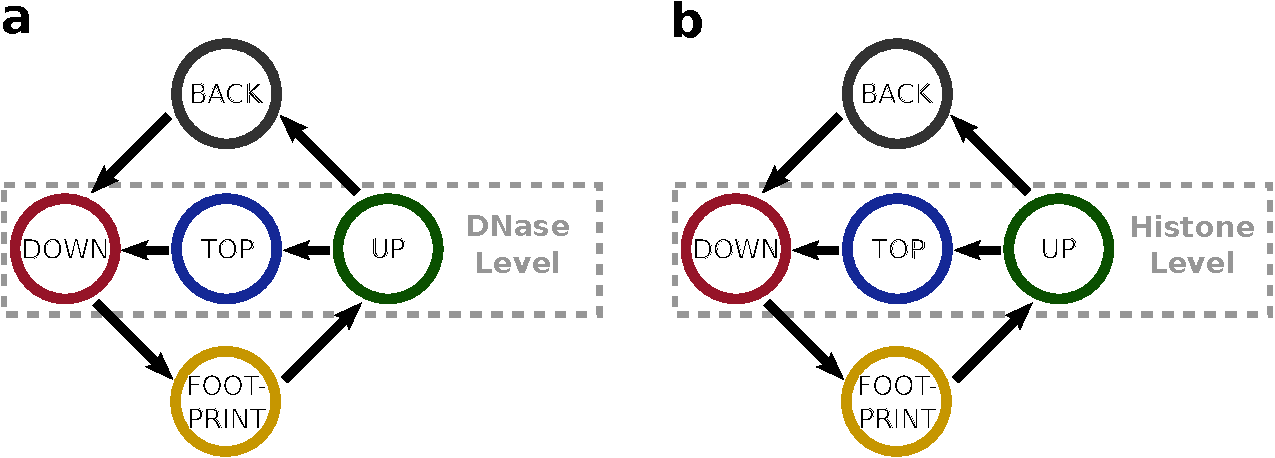
\includegraphics[width=0.99\textwidth]{gusmao_alternative_hmm}
%\caption[Alternative HMM topologies for single signal type input]{\textbf{Alternative HMM topologies for single signal type input.} (\textbf{a}) HMM topology which uses only DNase-seq signal as input. (\textbf{b}) HMM topology which uses only histone modification ChIP-seq signal.}
%\label{fig:gusmao_alternative_hmm}
%\end{figure}

%%%%%%%%%%%%%%%%%%%%%%%%%%%%%%%%%%%%%%%%%%%%%%%%%%%%%%%%%%%%%%%%%%%%%
% Section: Signal Processing Filters
%%%%%%%%%%%%%%%%%%%%%%%%%%%%%%%%%%%%%%%%%%%%%%%%%%%%%%%%%%%%%%%%%%%%%
\section{Signal Processing Filters}
\label{sec:signal.processing.filters}

% Introduction
In signal processing, a filter works by removing from a signal unwanted components or features. More formally, a filter is a device or process that works by removing or attenuating a certain number of harmonics from a signal and thus allows us to process the signal as required. All the signal processing filter theory presented here is based on the work by Lyons et al.~\cite{lyons2010}.

% Network synthesis filters
In this work we will explore four types of filters designed through network synthesis: (1) the Butterworth filter, (2) the Chebyshev filter, (3) the Elliptic filter and (4) the Bessel filter. The task of computational footprinting can be performed using filters by processing the genomic signals from DNase-seq and histone modification ChIP-seq in order to make the peak-dip-peak pattern more pronounced and applying a standard-deviation based windowing approach in order to detect these regions. Furthermore, the signal processing is able to smoothen the base pair resolution genomic signals without losing to much information and does not suffer from the same time-series processing biases as the hidden Markov model approach (Section~\ref{sec:hidden.markov.models}). Briefly, this approach is a simplified version of the HMM-based approach in order to test claims made that simpler methods might be preferable in terms of performance as more complex methods~\cite{cuellar2012,he2014}.

% This section
This section is divided into two parts. First we describe the basic definition of the signal processing filters that are used in this work (Section~\ref{sec:intro.signal.processing.filters}). Second, we describe how we used these filters along with a standard-deviation windowing approach in order to perform computational footprinting (Section~\ref{sec:computational.footprinting.filters}).

%%%%%%%%%%%%%%%%%%%%%%%%%%%%%%%%%%%%%%%%%%%%%%%%%%%%%%%%%%%%%%%%%%%%%
% Section: Introduction to Signal Processing Filters
%%%%%%%%%%%%%%%%%%%%%%%%%%%%%%%%%%%%%%%%%%%%%%%%%%%%%%%%%%%%%%%%%%%%%
\subsection{Introduction to Signal Processing Filters}
\label{sec:intro.signal.processing.filters}

% Periodic functions
A periodic function is a function that repeats its values in regular intervals or periods. Any signal can be represented as a periofic function by using a sum of sine waves. An example is the Fourier series defined as
\begin{equation}
  \label{eq:fourrier}
  \begin{array}{lcl} 
    y(t) & = & a_0 / 2 + a_1 \sin(\omega t) + a_2 \sin(2 \omega t) + a_3 \sin(3 \omega t) + \dots + a_n \sin(n \omega t) \\
         & = & \sum_{k=1}^n a_k \sin(k \omega t),
  \end{array}
\end{equation}
where $ \langle a_0, \dots, a_n \rangle $ are the Fourier coefficients and $ \omega $ represents the frequency of such periodic series.

% Harmonics
If a signal is periodic with frequency $\omega$, the only frequencies composing the signal are integer multiples of $f$. These frequencies are called harmonics. The first harmonic is $\omega$, the second harmonic is $2 \omega$ and so forth. A random signal, such as the genomic signals produced with the DNase-seq or histone modification ChIP-seq technologies, may be, and generally is, composed of a large number of harmonics. The main goal of the signal processing filters presented here is to remove certain harmonics and, as a result, pronounce the peak-dip-peak patterns in order for them to be easily recognizable.

% Transfer function
In this work, the filters will be defined based on their transfer functions. The transfer function of a filter is most often defined in the domain of the complex frequencies $ s $. The back and forth passage to/from this domain is operated by the Laplace transform and its inverse. Therefore, in this section we define the input for the filter as $ \mathbf{Z} $, which corresponds to the Laplace transform of the normalized and slope genomic signals matrix $\mathbf{X}$. Given the representation of $\mathbf{X}$ as a response function $f(t)$, defined for all real-valued genomic coordinates $t \geq 0 $; the Laplace transform is the function $\mathscr{L}(s)$, which is a unilateral transform defined by
\begin{equation}
  \label{eq:laplace}
  \mathscr{L}(s) = \int_{0}^\infty e^{-st} f(t) \diff x,
\end{equation}
where $ s = \sigma + j \omega $ is the complex number frequency with real numbers $ \sigma $ and $ \omega $. Given these formalizations, we are able to define the transfer function $G(s)$ of a filter as the ratio of the output signal $ \mathbf{H}(s) $ to that of the Laplace-transformed input signal $ \mathbf{Z}(s) $ as a function of the complex frequency $s$
\begin{equation}
  \label{eq:transfer}
  G(s) = \frac{\mathbf{H}(s)}{\mathbf{Z}(s)}.
\end{equation}

% Practical terms
The Laplace transformation and filter's transfer function derivations are computationally solved problems for signals represented by periodic functions. Such implementations are out of scope of this work. For more information regarding such implementations, please refer to Lyons et al.~\cite{lyons2010}. In practical terms, we used the implementation of the filters described in this section available at MATLAB version R2015b.

% This section
In this introduction we will briefly discuss the types of filter with regard to which harmonics they remove (Section~\ref{sec:filter.types}). More specifically, we will define low-pass, high-pass and band-stop filters. Then, we will discuss four types of filters used in this work. These filters differ based on the shape of their frequency response and each one can be of the types discussed in Section~\ref{sec:filter.types}. These four filter types are: the Butterworth filter (Section~\ref{sec:butterworth.filter}), the Chebyshev filter (Section~\ref{sec:chebyshev.filter}), the Elliptic filter (Section~\ref{sec:elliptic.filter}) and (4) the Bessel filter (Section~\ref{sec:bessel.filter}).

%%%%%%%%%%%%%%%%%%%%%%%%%%%%%%%%%%%%%%%%%%%%%%%%%%%%%%%%%%%%%%%%%%%%%
% Section: Filter Types
%%%%%%%%%%%%%%%%%%%%%%%%%%%%%%%%%%%%%%%%%%%%%%%%%%%%%%%%%%%%%%%%%%%%%
\subsubsection{Filter Types}
\label{sec:filter.types}

% Introduction
There are multiple ways to classify signal processing filters. Here, we focus on the classification based on the harmonic types the filters remove from a given signal. In this work we will refer to these filter types:

% Filter definitions
\vspace{0.5cm}
\noindent
\textbf{Low-pass filter:} \emph{A filter that passes signals with a frequency lower than a certain cutoff frequency and attenuates signals with frequencies higher than the cutoff frequency.}

\noindent
\textbf{High-pass filter:} \emph{A filter that passes signals with a frequency higher than a certain cutoff frequency and attenuates signals with frequencies lower than the cutoff frequency.}

\noindent
\textbf{Band-stop filter:} \emph{A filter that passes most frequencies unaltered, but attenuates those in a specific range to very low levels.}
\vspace{0.45cm}

% Practise
In practise, removing high frequency harmonics tends to smoothen the signal as high frequency harmonics tend to be more erratic than low frequency harmonics. On the other hand removing low frequency harmonics tends to make the signal much more pronounced. The amount of attenuation for each frequency depends on the filter design.

%%%%%%%%%%%%%%%%%%%%%%%%%%%%%%%%%%%%%%%%%%%%%%%%%%%%%%%%%%%%%%%%%%%%%
% Section: Butterworth Filter
%%%%%%%%%%%%%%%%%%%%%%%%%%%%%%%%%%%%%%%%%%%%%%%%%%%%%%%%%%%%%%%%%%%%%
\subsubsection{Butterworth Filter}
\label{sec:butterworth.filter}

% Butterworth Filter
The rationale behind the butterworth filter is that an ideal signal processing filter should not only completely reject the unwanted frequencies but should also have uniform sensitivity for the wanted frequencies. Such an ideal filter can not be achieved but it can be shown that successively closer approximations are obtained with increasing numbers of filter elements of the right values. It was shown that a low-pass filter could be designed whose cutoff frequency was normalized to $1$ radian per time unit and whose frequency response (gain) was
\begin{equation}
  \label{eq:butterworth1}
  G_n(\omega) = \sqrt{\frac{1}{{1+\omega^{2n}}}},
\end{equation}
where $ \omega $ is the angular frequency in radians per time unit $ t $ (which corresponds to our genomic coordinates) and $n$ is the number of poles in the filter.

%%%%%%%%%%%%%%%%%%%%%%%%%%%%%%%%%%%%%%%%%%%%%%%%%%%%%%%%%%%%%%%%%%%%%
% Section: Chebyshev Filter
%%%%%%%%%%%%%%%%%%%%%%%%%%%%%%%%%%%%%%%%%%%%%%%%%%%%%%%%%%%%%%%%%%%%%
\subsubsection{Chebyshev Filter}
\label{sec:chebyshev.filter}

% Chebyshev Filter
The Chebyshev filter allows for variation near the passband around the cutoff, which allows a much better roll off. Thus, it can accurately remove the unwanted frequencies but at the cost of inaccuracy near the cutoff region for the pass band frequency. More formally, Chebyshev filters have the property that they minimize the error between the idealized and the actual filter characteristic over the range of the filter but with ripples in the passband.

% Chebyshev filter type I
There are two possible implementations of the chebyshev filters, termed type I and II. In this work we focus on the type I Chebyshev filter, since it does roll off faster than the type II. Furthermore, the type II require more components, which makes the parameters selection more difficult and more prone to overfitting.

% Transfer function
The Chebyshev type I transfer function is defined as
\begin{equation}
  \label{eq:chebyshev1}
  G_n(\omega) = \frac{1}{\sqrt{1+{\epsilon^2 {T}_{n}^{2} (\frac{\omega}{\omega_0})}}},
\end{equation}
where $ \omega $ is the angular frequency in radians per time unit $ t $ (which corresponds to our genomic coordinates), $n$ is the number of poles in the filter, $ \epsilon $ is the ripple factor, $ \omega_0 $ is the cutoff frequency and $ T_n $ is a Chebyshev polynomial of the $n^{\text{th}}$-order.

%%%%%%%%%%%%%%%%%%%%%%%%%%%%%%%%%%%%%%%%%%%%%%%%%%%%%%%%%%%%%%%%%%%%%
% Section: Elliptic Filter
%%%%%%%%%%%%%%%%%%%%%%%%%%%%%%%%%%%%%%%%%%%%%%%%%%%%%%%%%%%%%%%%%%%%%
\subsubsection{Elliptic Filter}
\label{sec:elliptic.filter}

% Introduction
An elliptic filter is a signal processing filter with equalized ripple behavior in both the passband and the stopband. The amount of ripple in each band is independently adjustable, and no other filter of equal order can have a faster transition in gain between the passband and the stopband, for the given values of ripple (whether the ripple is equalized or not). Alternatively, one may give up the ability to adjust independently the passband and stopband ripple, and instead design a filter which is maximally insensitive to component variations.

% Similarity to Butterworth and Chebyshev
As the ripple in the stopband approaches zero, the filter becomes a type I Chebyshev filter. As the ripple in the passband approaches zero, the filter becomes a type II Chebyshev filter and finally, as both ripple values approach zero, the filter becomes a Butterworth filter.

% Elliptic Filter
More formally, the gain of the elliptic filter is given by
\begin{equation}
  \label{eq:elliptic1}
  G_n(\omega)=\frac{1}{\sqrt{1+{ \epsilon^2 R_n^2(\xi,\omega/\omega_0)}}},
\end{equation}
where $ \omega $ is the angular frequency in radians per time unit $ t $ (which corresponds to our genomic coordinates), $n$ is the number of poles in the filter, $ \epsilon $ is the ripple factor, $ \omega_0 $ is the cutoff frequency, $ \xi $ is the selectivity factor and $ R_n $ is the $n^{\text{th}}$-order elliptic rational function.

%%%%%%%%%%%%%%%%%%%%%%%%%%%%%%%%%%%%%%%%%%%%%%%%%%%%%%%%%%%%%%%%%%%%%
% Section: Bessel Filter
%%%%%%%%%%%%%%%%%%%%%%%%%%%%%%%%%%%%%%%%%%%%%%%%%%%%%%%%%%%%%%%%%%%%%
\subsubsection{Bessel Filter}
\label{sec:bessel.filter}

% Bessel Filter
The Bessel filter is a signal processing filter with a maximally flat group/phase delay (maximally linear phase response), which preserves the wave shape of filtered signals in the passband. More formally, the Bessel filter can be characterized as
\begin{equation}
  \label{eq:bessel1}
  G_n(\omega) = \frac{\theta_n(0)}{\theta_n(\omega/\omega_0)},
\end{equation}
where $ \omega $ is the angular frequency in radians per time unit $ t $ (which corresponds to our genomic coordinates), $n$ is the number of poles in the filter, $ \omega_0 $ is the cutoff frequency and $ \theta_n(s) $ is the $n^{\text{th}}$-order reverse Bessel polynomial.

%%%%%%%%%%%%%%%%%%%%%%%%%%%%%%%%%%%%%%%%%%%%%%%%%%%%%%%%%%%%%%%%%%%%%
% Section: Computational Footprinting with Filters
%%%%%%%%%%%%%%%%%%%%%%%%%%%%%%%%%%%%%%%%%%%%%%%%%%%%%%%%%%%%%%%%%%%%%
\subsection{Computational Footprinting with Filters}
\label{sec:computational.footprinting.filters}

% Introduction
As previously mentioned, the rationale of the signal processing filters for computational footprinting is to remove inadequate frequencies in order to make the DNase-seq and histone modification peaks more pronounced and detectable by simpler window-based approaches. The input for all filters are the matrix of normalized DNase-seq and histone modification ChIP-seq signals, transformed in order to fit the signal's implementations, as described in Section~\ref{sec:intro.signal.processing.filters}.

% Brief method description
The method works as follows. First, we detect regions enriched with the combination of DNase-seq and histone modification ChIP-seq signal as described in Section~\ref{sec:selection.genomic.regions}. Then, we apply the filtering techniques within these regions using MATLAB version R2015b (``Signal Filtering''). Finally, we apply a standard deviation-based windowing approach to detect the significant depletions in the data, i.e. the footprint pattern (``Standard Deviation Footprinting'').

%%%%%%%%%%%%%%%%%%%%%%%%%%%%%%%%%%%%%%%%%%%%%%%%%%%%%%%%%%%%%%%%%%%%%
% Section: Signal Filtering
%%%%%%%%%%%%%%%%%%%%%%%%%%%%%%%%%%%%%%%%%%%%%%%%%%%%%%%%%%%%%%%%%%%%%
\subsubsection{Signal Filtering}
\label{sec:signal.filtering}

% Signal filtering 1
For each genomic region enriched for the selected genomic features, we applied the filters described in Section~\ref{sec:intro.signal.processing.filters}. Different filters with different parameterizations provide different accuracies. The parameterization will be explored in Section~\ref{sec:filters.parameterization}. The implementation of these filters are made simple using the MATLAB tool. Within this framework we are able to perform the signal frequency and time-domain transformations. For every filter, we applied the implementations of their high-pass, low-pass and band-stop filters: (1) the high-pass filter removes background noise in the data; (2) the low-pass filter attenuates the peaks in the genomic signal and (3) band-stop filter normalize the signals in order to prepare them for the standard deviation-based footprinting.

% Signal filtering 2
Such three-filter approach is possible given the fact that there is no stability danger since we are not bound by hardware-implementation of the filters. Such implementation provides a significant filtering roll off, which depends only on the parameter selection for each filter type.

% Signal filtering 3
Finally, all filters output real-valued signals which contains negative values. In order to prevent numerical problems on the standard deviation-based footprinting which these negative values might cause, we evaluated the global minimum value and summed the absolute version of this value for all values of the genomic signal.

%%%%%%%%%%%%%%%%%%%%%%%%%%%%%%%%%%%%%%%%%%%%%%%%%%%%%%%%%%%%%%%%%%%%%
% Section: Standard Deviation Footprinting
%%%%%%%%%%%%%%%%%%%%%%%%%%%%%%%%%%%%%%%%%%%%%%%%%%%%%%%%%%%%%%%%%%%%%
\subsubsection{Standard Deviation Footprinting}
\label{sec:standard.deviation.footprinting}

% Experimental standard deviation
The second part of the method corresponds to the statistical analysis of the filtered signal to obtain the footprint predictions. First, we measured the average standard deviation within the filtered signal for: (1) a $20$ bp window centered at the beginning of all true MPBSs in the human chromosome~1, (2) a $20$ bp window centered at the ending of all true MPBSs in the human chromosome~1. We call these values, respectively $ \bar{\alpha} $ and $ \bar{\beta} $. We considered all MPBSs obtained by applying motif matching in cell type K562 and we considered the true MPBS the ones that contained ChIP-seq evidence (see Section~\ref{sec:chipseq.evaluation}). The human chromosome~1 was removed from all subsequent evaluation experiments.

% Standard deviation footprinting
Then, we are able to perform a window-based search within the genomic signal for $ k $ bp regions in which the standard deviation evaluated at a $20$ bp window from the region's start site (and region's end site) does not excede a certain threshold value $ \hat{\alpha} $ (and $ \hat{\beta} $) from the experimentally-evaluated standard deviations $ \bar{\alpha} $ (and $ \bar{\beta} $). Such approach consists on a slightly modified version of the algorithm proposed by Neph et al.~\cite{neph2012a}. Such modifications were performed in order to fit the filtered signals. The standard deviations are evaluated dynamically as the window slides within the selected regions. Finally, different values of $ k $, $ \bar{\alpha} $ and $ \bar{\beta} $ produces different results. A full experimental parameter selection description is available in Section~\ref{sec:filters.parameterization}

%%%%%%%%%%%%%%%%%%%%%%%%%%%%%%%%%%%%%%%%%%%%%%%%%%%%%%%%%%%%%%%%%%%%%
% Section: Statistical Methods
%%%%%%%%%%%%%%%%%%%%%%%%%%%%%%%%%%%%%%%%%%%%%%%%%%%%%%%%%%%%%%%%%%%%%
\section{Statistical Methods}
\label{sec:statistical.methods}

% Comparison between competing methods
All method comparison in this work are performed using the non-parametric Friedman-Nemenyi hypothesis test~\cite{demsar2006}. Such test provides a rank of the methods as well as the statistical significance of whether a particular method was outperformed.

% Correlation
All correlations evaluated in this work are based on the Spearman's rank correlation coefficient (denoted as $r$).

% Statistical test on diff between two samples
All differences between the distribution of two samples (or more samples however in a pair-wise way) are analyzed using the non-parametric Mann–Whitney–Wilcoxon hypothesis test (also known as Mann–Whitney U test, Wilcoxon rank-sum test or Wilcoxon–Mann–Whitney test). The only exception is regarding the FLR-Exp evaluation approach (see Section~\ref{sec:flrexp.evaluation}), in which the Kolmogorov-Smirnoff hypothesis test was used, in accordance to Yard{\i}mc{\i} et al.\cite{yardimci2014}.

% Multiple test correction
All $p$-values are corrected for multiple comparisons using the Benjamini and Hochberg method~\cite{benjamini1995} (also known as false discovery rate (FDR) control method).

% Sensitivity (recall), specificity and precision
Receiver operating characteristic (ROC) curves and precision-recall (PR) curves will be used to evaluate methods using the ChIP-seq evaluation approach (see Section~\ref{sec:chipseq.evaluation}). More specifically, we use the area under the ROC curve (AUC) and area under the PR curve (AUPR) to assess the performance of the methods in predicting cell-specific (active) transcription factor binding sites. Given a rank of footprint predictions, the ROC curve can be evaluated by measuring the sensitivity decrease as the specificity increases and the precision-recall curve can be evaluated by measuring the variations in the precision as the recall (sensitivity) increases. The sensitivity (recall), specificity and precision can be written as
\begin{equation}
  \label{eq:baseline.statistics}
  \begin{array}{lcl}
    \text{sensitivity} = \frac{\text{TP}}{\text{TP}+\text{FN}}, \\[1.2em]
    \text{specificity} = \frac{\text{TN}}{\text{TN}+\text{FP}}, \\[1.2em]
    \text{precision} = \frac{\text{TP}}{\text{TP}+\text{FP}},
  \end{array}
\end{equation}
where $ \text{TP} $ represents the true positives, $ \text{FP} $ represents the false positives, $ \text{TN} $ represents the true negatives and $ \text{FN} $ represents the false negatives.

%%%%%%%%%%%%%%%%%%%%%%%%%%%%%%%%%%%%%%%%%%%%%%%%%%%%%%%%%%%%%%%%%%%%%
% Section: Discussion
%%%%%%%%%%%%%%%%%%%%%%%%%%%%%%%%%%%%%%%%%%%%%%%%%%%%%%%%%%%%%%%%%%%%%
\section{Discussion}
\label{sec:discussion.3}

% Discussion
In this chapter we presented the methods we devised to perform the prediction of active transcription factor binding sites using DNase-seq and histone modification ChIP-seq data. First we described the creation and processing of the genomic signals used as input for the methods. Then, we introduced, formalized and show the practical application of two proposed methodologies: (1) the HMM-based computational footprinting approach and the (2) signal processing filter-based computational footprinting approach. Finally, we closed the chapter by describing all the statistical techniques used to assess method performance and the significance of statistical tests which are performed on later chapters. 


